\chapter{More on Bonding, XeF$_n$, O$_3$}

\section{Noble Gas Fluorides}

In Chapter 9, we saw that HeH, NeH, and ArH could not make a three-electron 
bond because two electrons in a bonding orbital and one electron in an 
antibonding orbital lead to
\begin{equation}
\left( \ell + r \right)^2 \left( \ell - r \right) = {1 \over 2} 
HeH + {1 \over 2} He^+H^-
\label{chap11-eqno1}
\end{equation}
where $He^+H^-$ is a very high energy configuration.  Although the above 
reasoning is true, we can find an exception by replacing He with an atom 
such as Xe that is much easier to ionize, and by
replacing H with an atom such as F that is much more electronegative.

\subsection{AF$_2$}

\begin{table}
\caption{ Estimated bond energy, in eV, for linear $FAF$ 
using the ionic model $FA^+F^-$.}
\label{chap11-tab1}
\begin{tabular}{ccccccc}\\ \hline
& He & Ne & Ar & Kr & Xe & Rn\cr

$IP(A)$ & 24.587 & 21.564 & 15.759 & 13.999 & 12.130 & 10.748\cr
$IP(A)-EA(F)^f$ & 21.19 & 18.17 & 12.36 & 10.60 & 8.73 & 7.35\cr
$R(A^+-F^-)$ & (1.3) & (1.41) & (1.73) & 1. 875$^e$ & 1.977 & 
(1.98)\cr
$E(A^+F^-)-E(A)-E(F)$ & 10.11 & 7.95 & 4.04 & 2.92 & 1.45 & 0.08\cr
$D(F-A^+)$ & (5.9)$^c$ & 1.60$^a$ & 2. 62$^a$ & 2. 55$^{a,d}$ & 
2.88$^{a,d}$ & (2.7)$^b$\cr
$E(FA^+F^-)-E(A)-2E(F)$ & +4.2 & +6.4 & +1.4 & +0.3 & $-$1.4 & 
$-$2.6\cr
Resonance & 1 & 1 & 1 & 1 & 1 & 1\cr
Bond Energy $(AF_2)$ & $-$3.2 & $-$5.4 & $-$0.4 & 0.7 & 2.4 & 3.6\cr
Experiment$^g$ & - & - & - & 0.95 & 2.69\cr
\hline
\end{tabular}\\
$^a$ Based on bond energy of corresponding halogen-fluoride, for 
example, $D(IF) = 2.88$ eV.
$^b$ An average of the values for Ar, Kr, and Xe. 
$^c$ Based on $D(HF)$. 
$^d$ Experimental values are
$D(KrF^+) \approx 2$ eV, and $D(XeF^+) \approx 1.6$ eV. 
$^e$ Experimental value is $R(KrF^+) = 1.752$ \AA. 
$^f$ Using $EA(F) = 3. 399$. 
$^g$ Cotton and Wilkenson, page 587.
\end{table}

In Table \ref{chap11-tab1}, we calculate the energetics for forming
the molecule $A^+F^-$, where the energy, in eV, is calculated as
\begin{equation}
E(A^+F^-) = E(A) + E(F) + IP(A) - EA(F) - {14.4 \over R(A)}
\label{chap11-eqno2}
\end{equation}
Here, we see that the estimated charge transfer species are unstable with 
respect to the free atoms by 10.1 eV for He, 8.0 eV for Ne, 4.0 eV for 
Ar, 2.9 eV for Kr, 1.5 eV for Xe, and 0.1 eV for Rn.  Both KrF and XeF 
are known to form only very weak, very long bonds, $\sim$0.1
to 0.2 eV, in agreement with these results.  Consider, however, the 
orbitals for the $A^+F^-$ species,
\begin{equation}
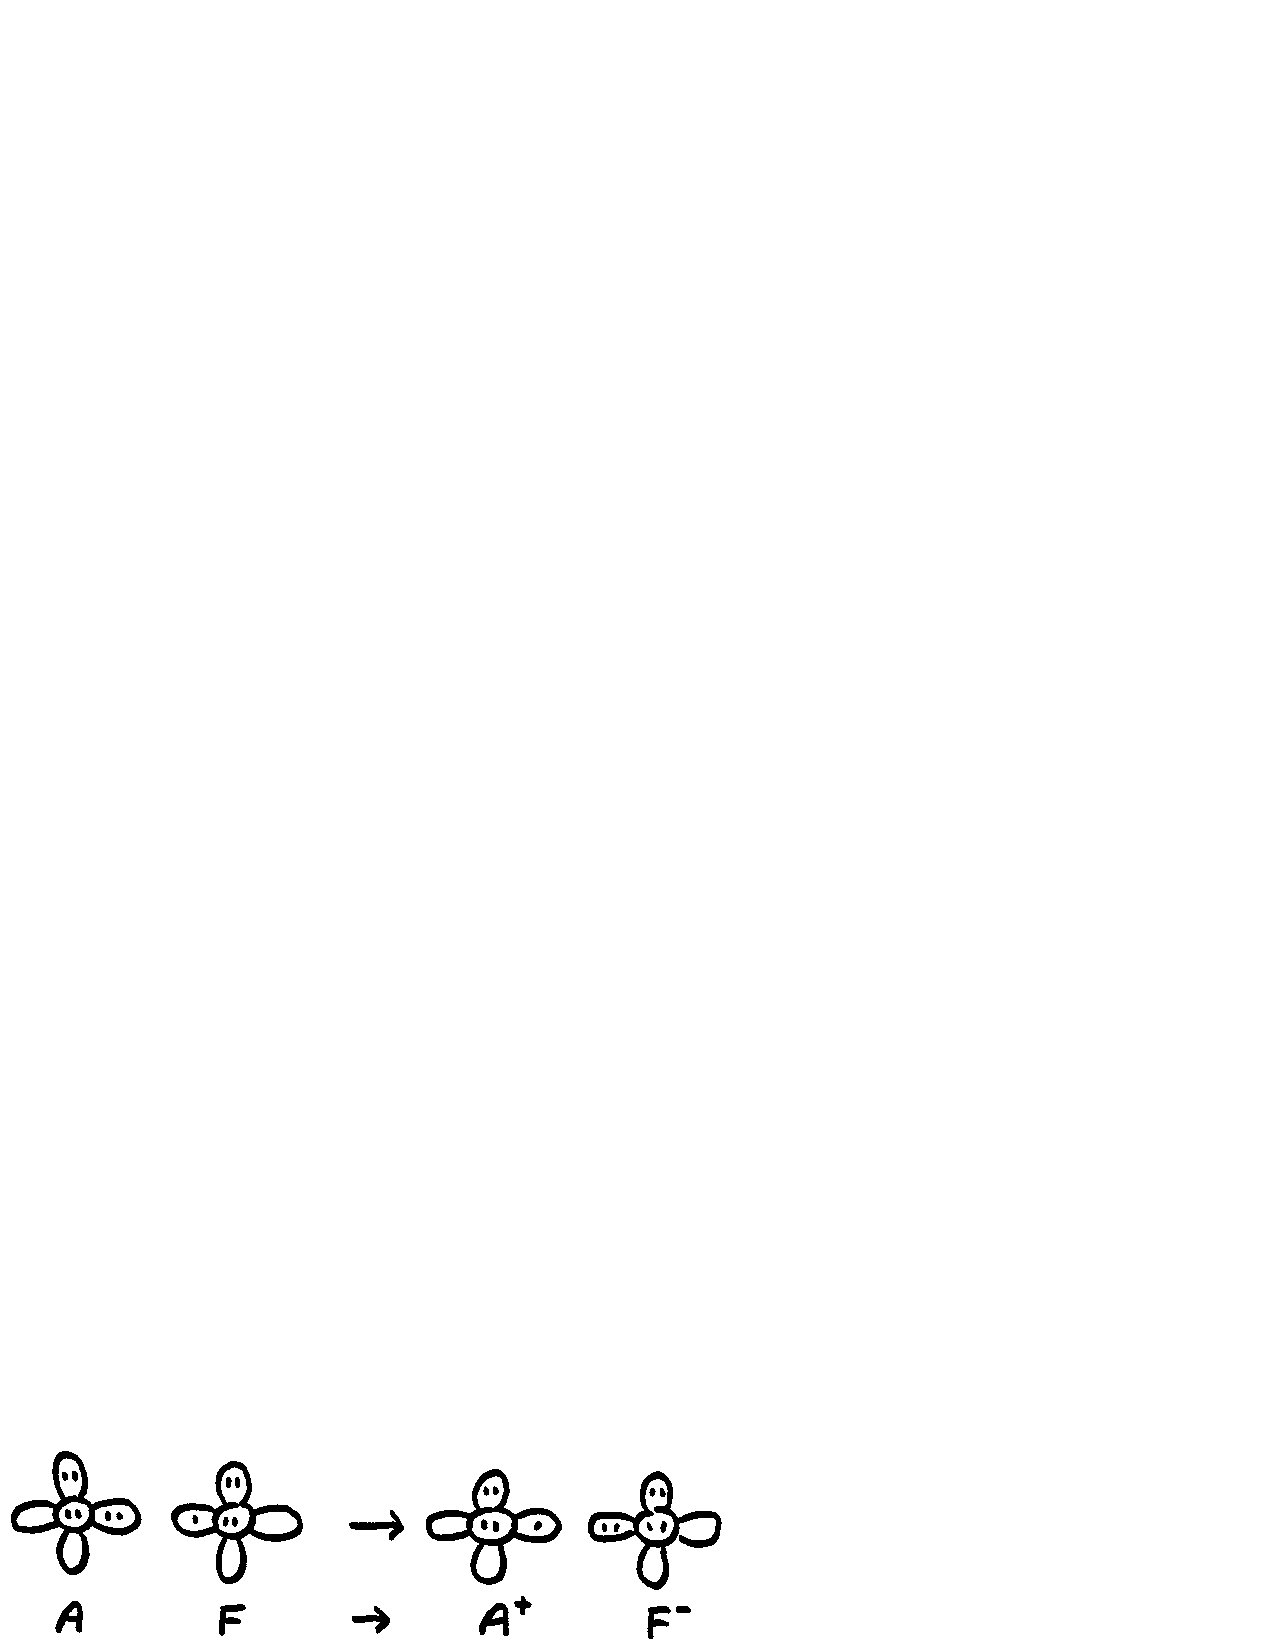
\includegraphics{fg11-a}
\label{chap11-eqno3}
\end{equation}
On the $A^+$ is a $p\sigma$ orbital aching to bond to some other 
orbital. Thus, if there is a second $F$ on
the opposite side of $A$, a linear $FAF$ system, then we get a covalent bond 
to this second $F$,
\begin{equation}
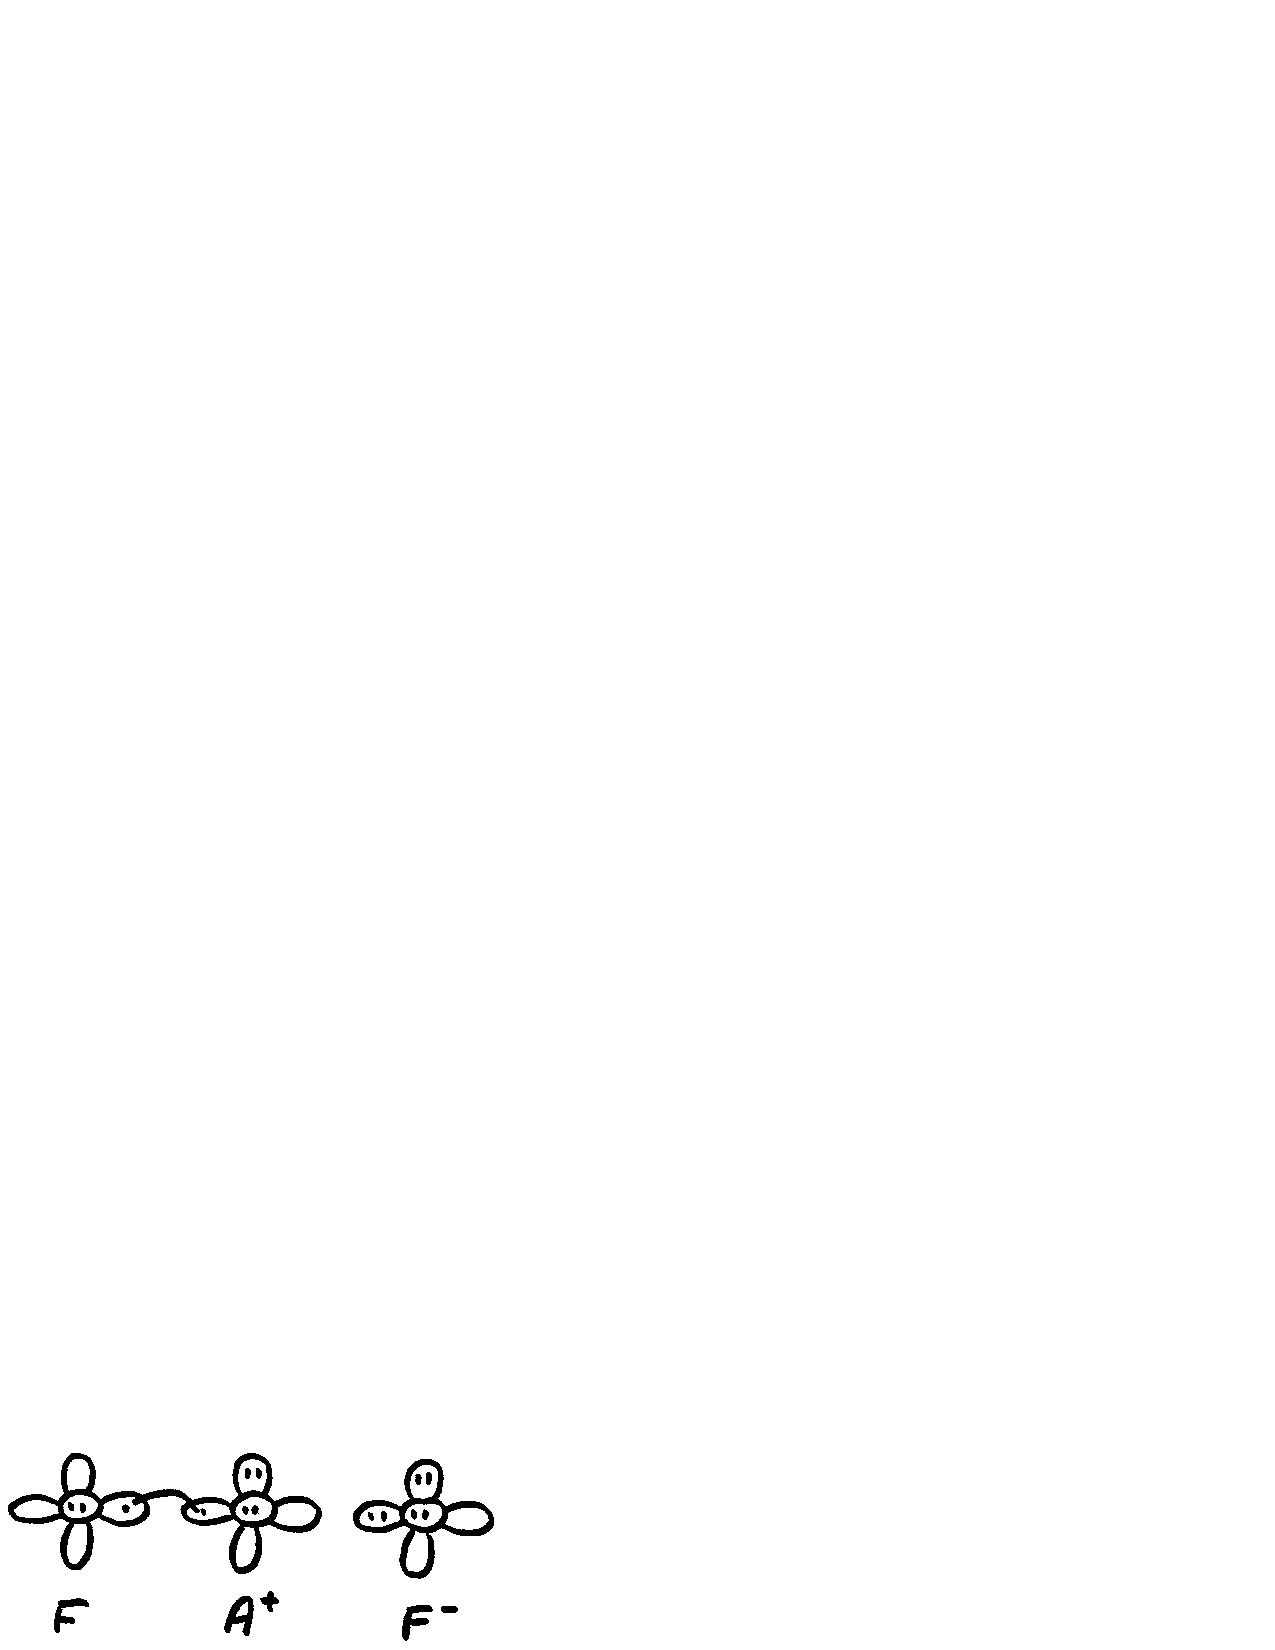
\includegraphics{fg11-b}
\label{chap11-eqno4}
\end{equation}
These estimates indicate that with bonding as in equation
(\ref{chap11-eqno4}), $RnF_2$ would be bound by 2.6 eV and $XeF_2$ by
1.4 eV.  Also, $KrF_2$ would only be unbound by 0.3 eV, but $ArF_2$,
$NeF_2$, and $HeF_2$ would be unbound by 1.4, 6.4, and 4.2 eV,
respectively. The configuration
\begin{equation}
F^- A^+ F
\end{equation}
is equivalent to equation (\ref{chap11-eqno4}), and we could expect a
resonance between these two configurations
\begin{equation}
F^- A^+ F + FA^+ F^-
\label{chap11-eqno5}
\end{equation}
to yield an energy about I eV lower.  Thus, we could expect a total bond 
energy of 3.6 eV for $RnF_2$, 2.4 eV for $XeF_2$, and 0.7 eV for $KrF_2$, 
but the other noble gas difluorides would be unstable.  Indeed, $XeF_2$ 
and $KrF_2$ have been synthesized and detected experimentally.

The bonding in $XeF_2$ requires both fluorines and involves four electrons 
distributed over the three $Xe$ and $F$ $p \sigma$ orbitals.  The $XeF_2$ 
bond involves all three configurations
\begin{equation}
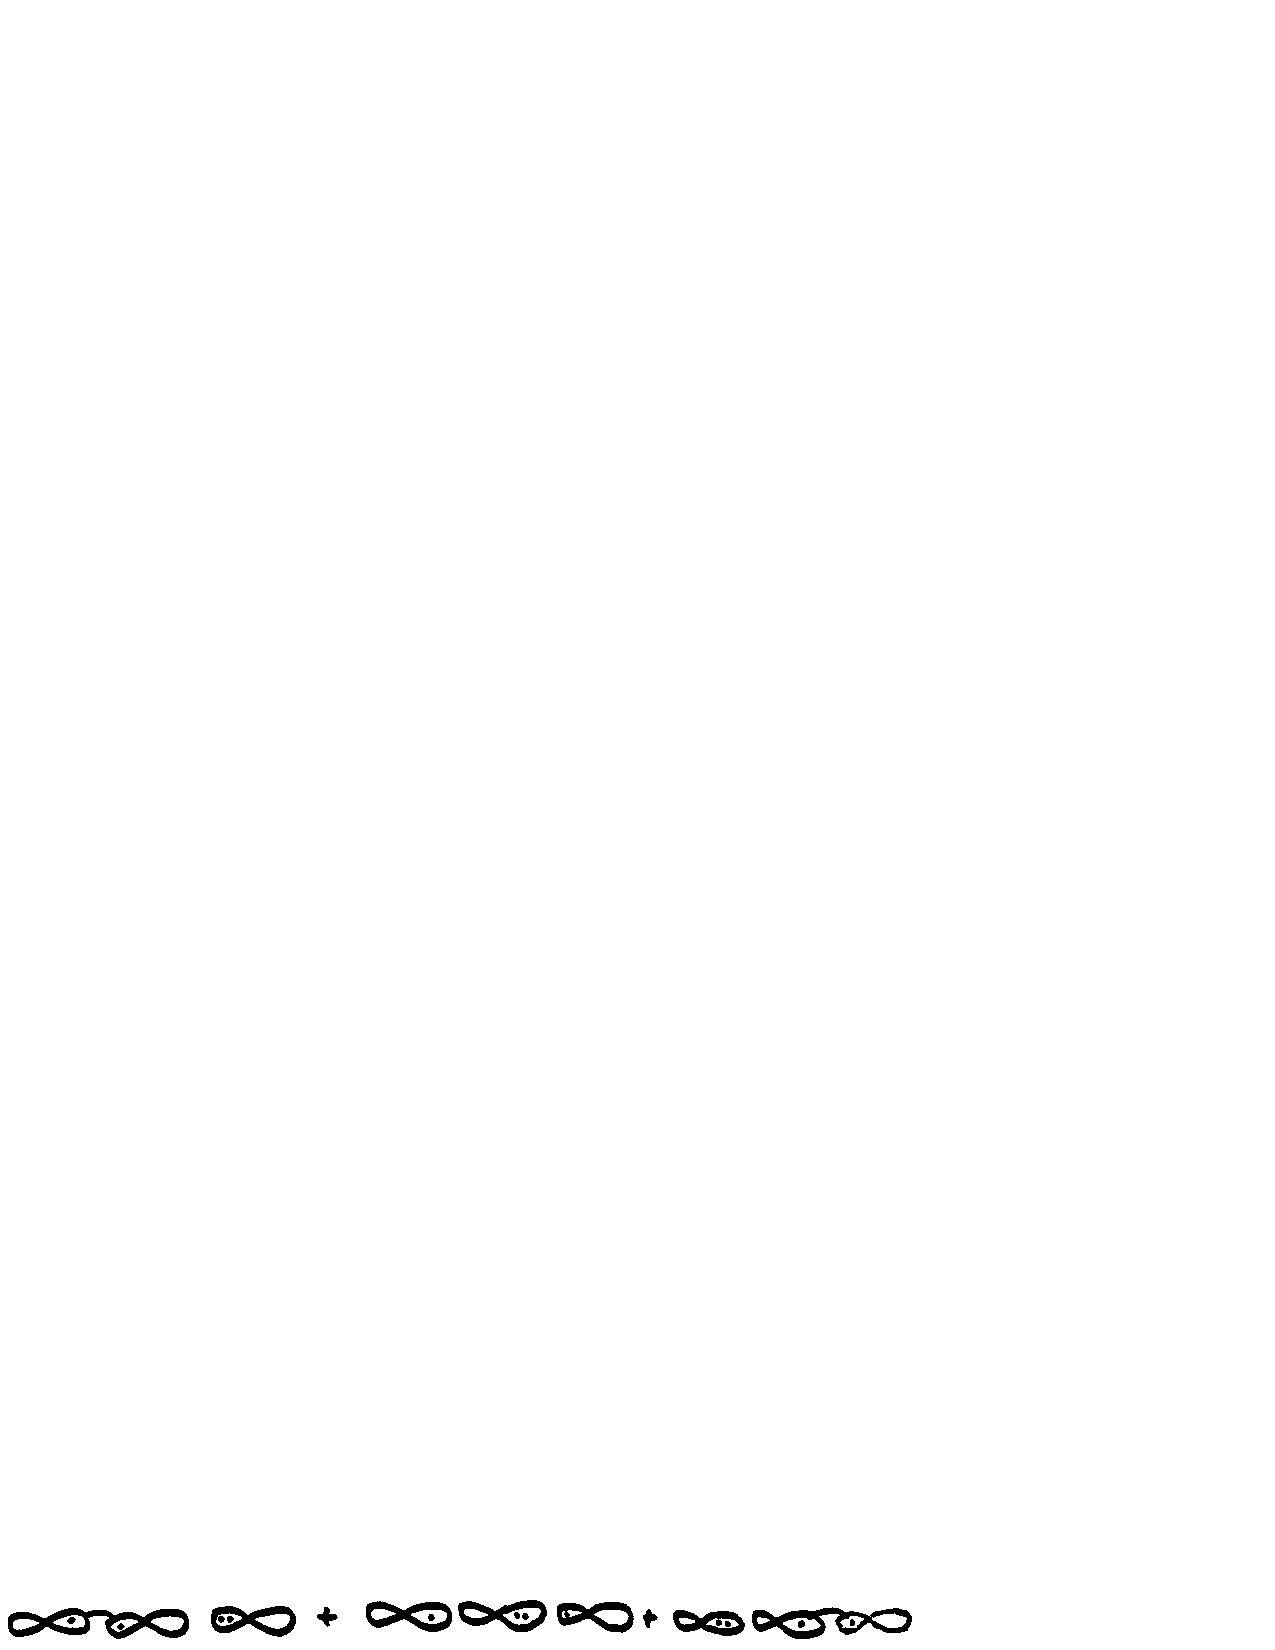
\includegraphics{fg11-c}
\label{chap11-eqno6}
\end{equation}
where pi orbitals have been deleted for clarity.  Rather than drawing all 
these resonance configurations, we will merely refer to this as the three-center, 
four-electron sigma bond, and we will schematically indicate it as
\begin{equation}
F \longleftarrow Xe	\longrightarrow F
\end{equation}
Notice that this bond needs to be linear in order to be able to get all 
three resonance structures.

\subsection{XeF$_4$ and XeF$_6$}

As one good turn deserves another, so a three-center, four-electron 
sigma bond involving one $p$ orbital on the Xe can be formed for all 
three $p$ orbitals. Thus $XeF_4$ is stable and square planar,
\begin{equation}
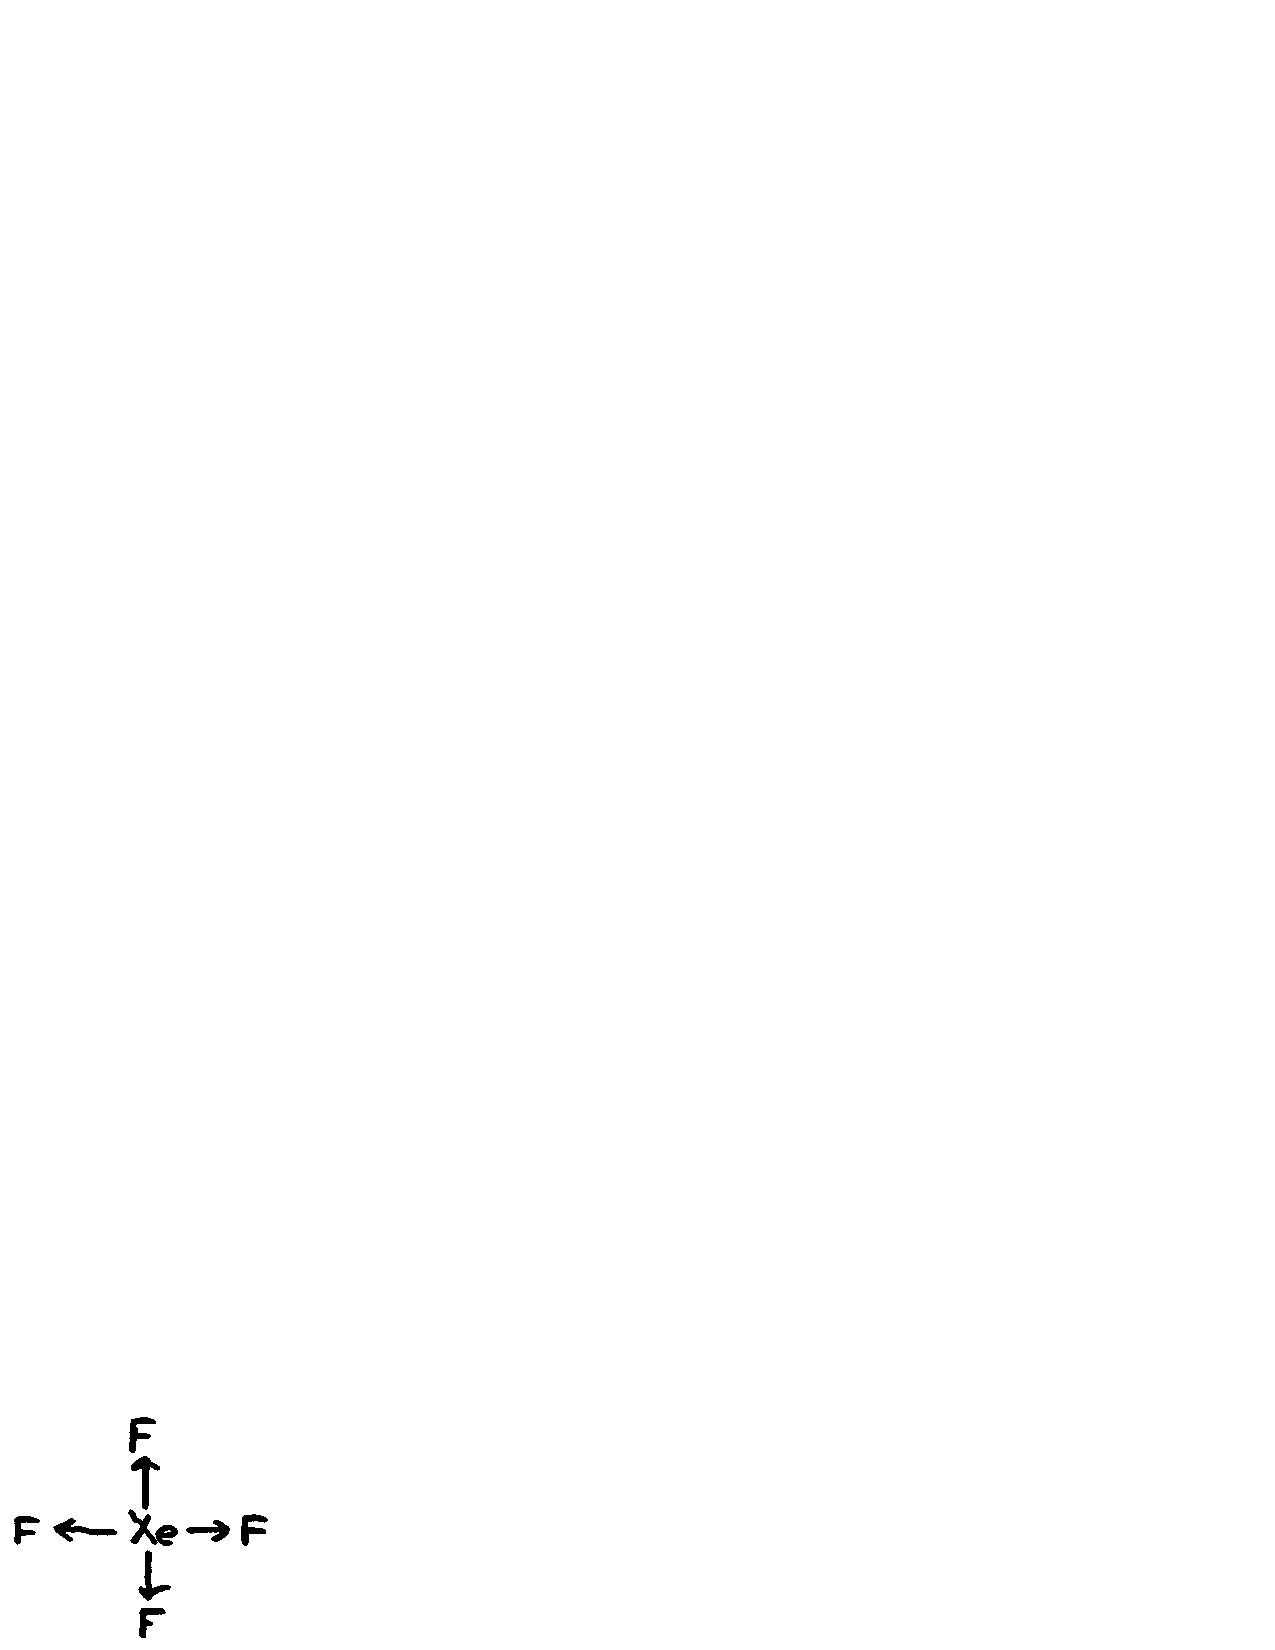
\includegraphics{fg11-d}
\label{chap11-eqno7}
\end{equation}
and $XeFe_6$ is stable and octahedral,
\begin{equation}
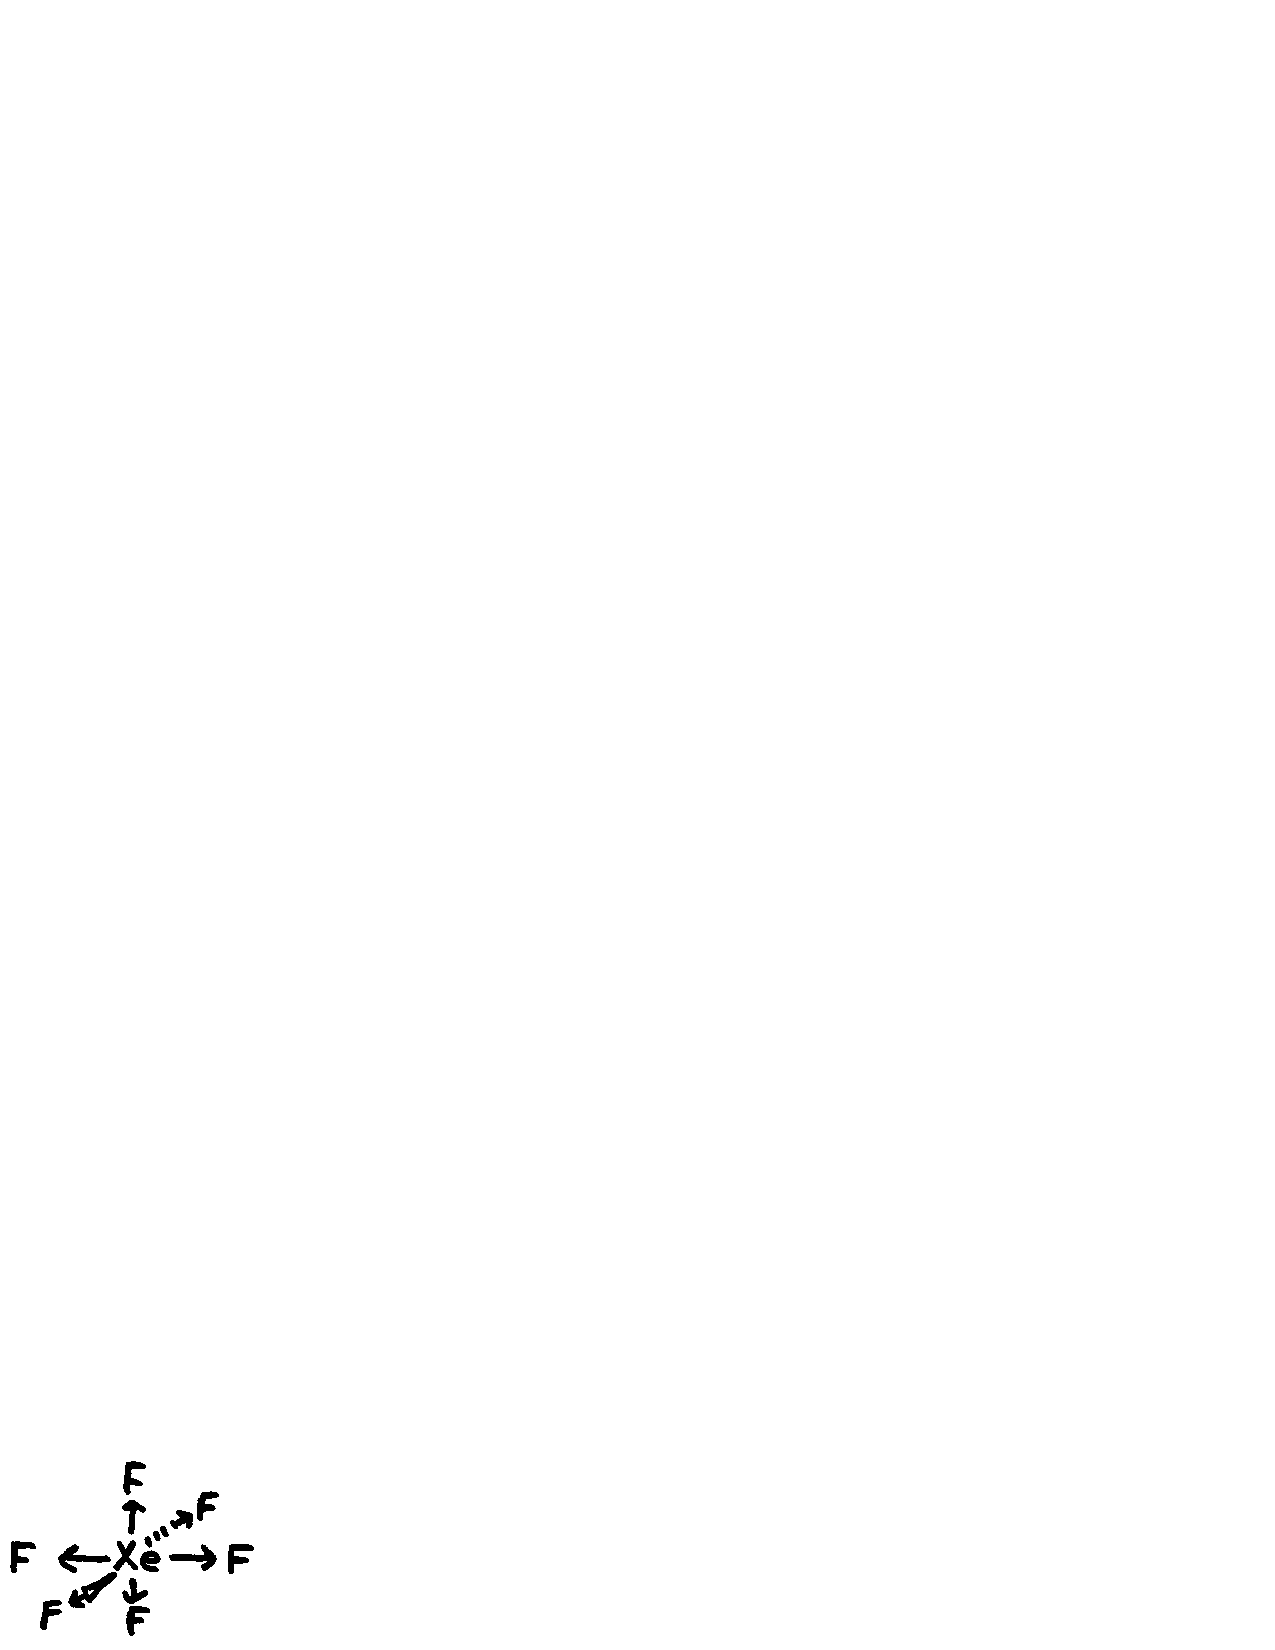
\includegraphics{fg11-e}
\label{chap11-eqno8}
\end{equation}

The total bond energy for crystalline $XeF_4$ is reported$^1$ as 6 eV, 
whereas an estimate for $XeF_2$ would suggest $\sim$4.8 eV for gaseous $XeF_4$.

\subsection{Stability}

\begin{table}
\caption{Estimated bond lengths for FAF.}
\label{chap11-tab2}
\begin{tabular}{ccccccc}\\ \hline
&He & Ne & Ar & Kr & Xe & Rn\cr
\noalign{\medskip\hrule\medskip}
${1 \over 2}$R(A$^+_2$) & 1.51 & 1.58 & 1.88 & 2.01 & 2.18\cr
R(halogen-fluoride) & 0.917 & 1.41 & 1.628 & 1.756 & 1.910\cr
R(AF$^+$) & & & & 1.752\cr
R(FAF) & & & & 1.875 & 1.977\cr
Estimated $R(FAF)$ & 1.3 & 1.41	& 1.73 & & & 1.98\cr
\hline
\end{tabular}
\end{table}

An important consideration in deciding when a species such as $XeF_2$
or $XeF_6$ can be formed is not just the total bond energy.  We must
consider the energetics for various decomposition products. Thus, the
bond energies of Table \ref{chap11-tab1} assume
\begin{equation}
AF_2 \longrightarrow A + F + F ,
\end{equation}
whereas, the final decomposition product would probably be
\begin{equation}
AF_2 \longrightarrow A + F_2 .
\end{equation}
Since the bond energy of $F_2$ is 1.6 eV, only $AF_2$ species with total bond 
energies greater than 1.6 eV are likely to be stable.  This leaves only 
$XeF_2$ and $RnF_2$, actually, $KrF_2$ has also been observed.

This raises an important point as to why $F$ is a good ligand. Using $EA(Cl) = 
3.615$ eV, $R(Xe^+Cl) \sim 2.32$ \AA, and $D(XeCl) = 2.15$ eV, we estimate 
that $XeCl_2$ is stable by 0.84 eV
with respect to Xe plus two Cl atoms. However, the bond energy of $Cl_2$ is 
2.48 eV, as compared with 1.60 eV for $F_2$, so that $XeCl_2$ would no 
doubt be too unstable to be isolated.

\section{Halogen Fluorides}

\subsection{ClF$_n$}

\begin{table}
\caption{Estimates of three-center, four-electron sigma 
bonds to ClF.}
\label{chap11-tab3}
\begin{tabular}{ccc}\\ \hline
& ClF & ClH\cr

IP(ClX) & 12.66 & 12.75\cr
IP-EA & 9.26 & 9.35\cr
R(ClF) & 1. 70\AA$^a$ & 1. 70\AA\cr
E(A$^+$F$^-$)$-$E(A)-E(F) & 0.79 & 0.88\cr
D(F $-$ Cl$^+$) & 2.6 & 2.62\cr
E[F(CIX)$^+$F$^-$]$-$2E(F)$-$E(ClX) & $-$1.83 & $-$1.74\cr
Resonance & $\sim$1 & $\sim$1\cr
Bond of two F to ClX\cr
~~~~~ Estimated & 2.8 & 2.7\cr
~~~~~ Experimental & 2.6\cr
\hline
\end{tabular}\\
$^a$ Experimental value for CIF$_3$.
\end{table}

In Chapter 6, we concluded that Cl could only bond to one H, this is
correct.  However, with fluorine ligands we can make bonds much as in
the noble gas fluorides.  Estimates analogous to Table
\ref{chap11-tab1} are made in Table \ref{chap11-tab3} where we expect $ClF_3$
\begin{equation}
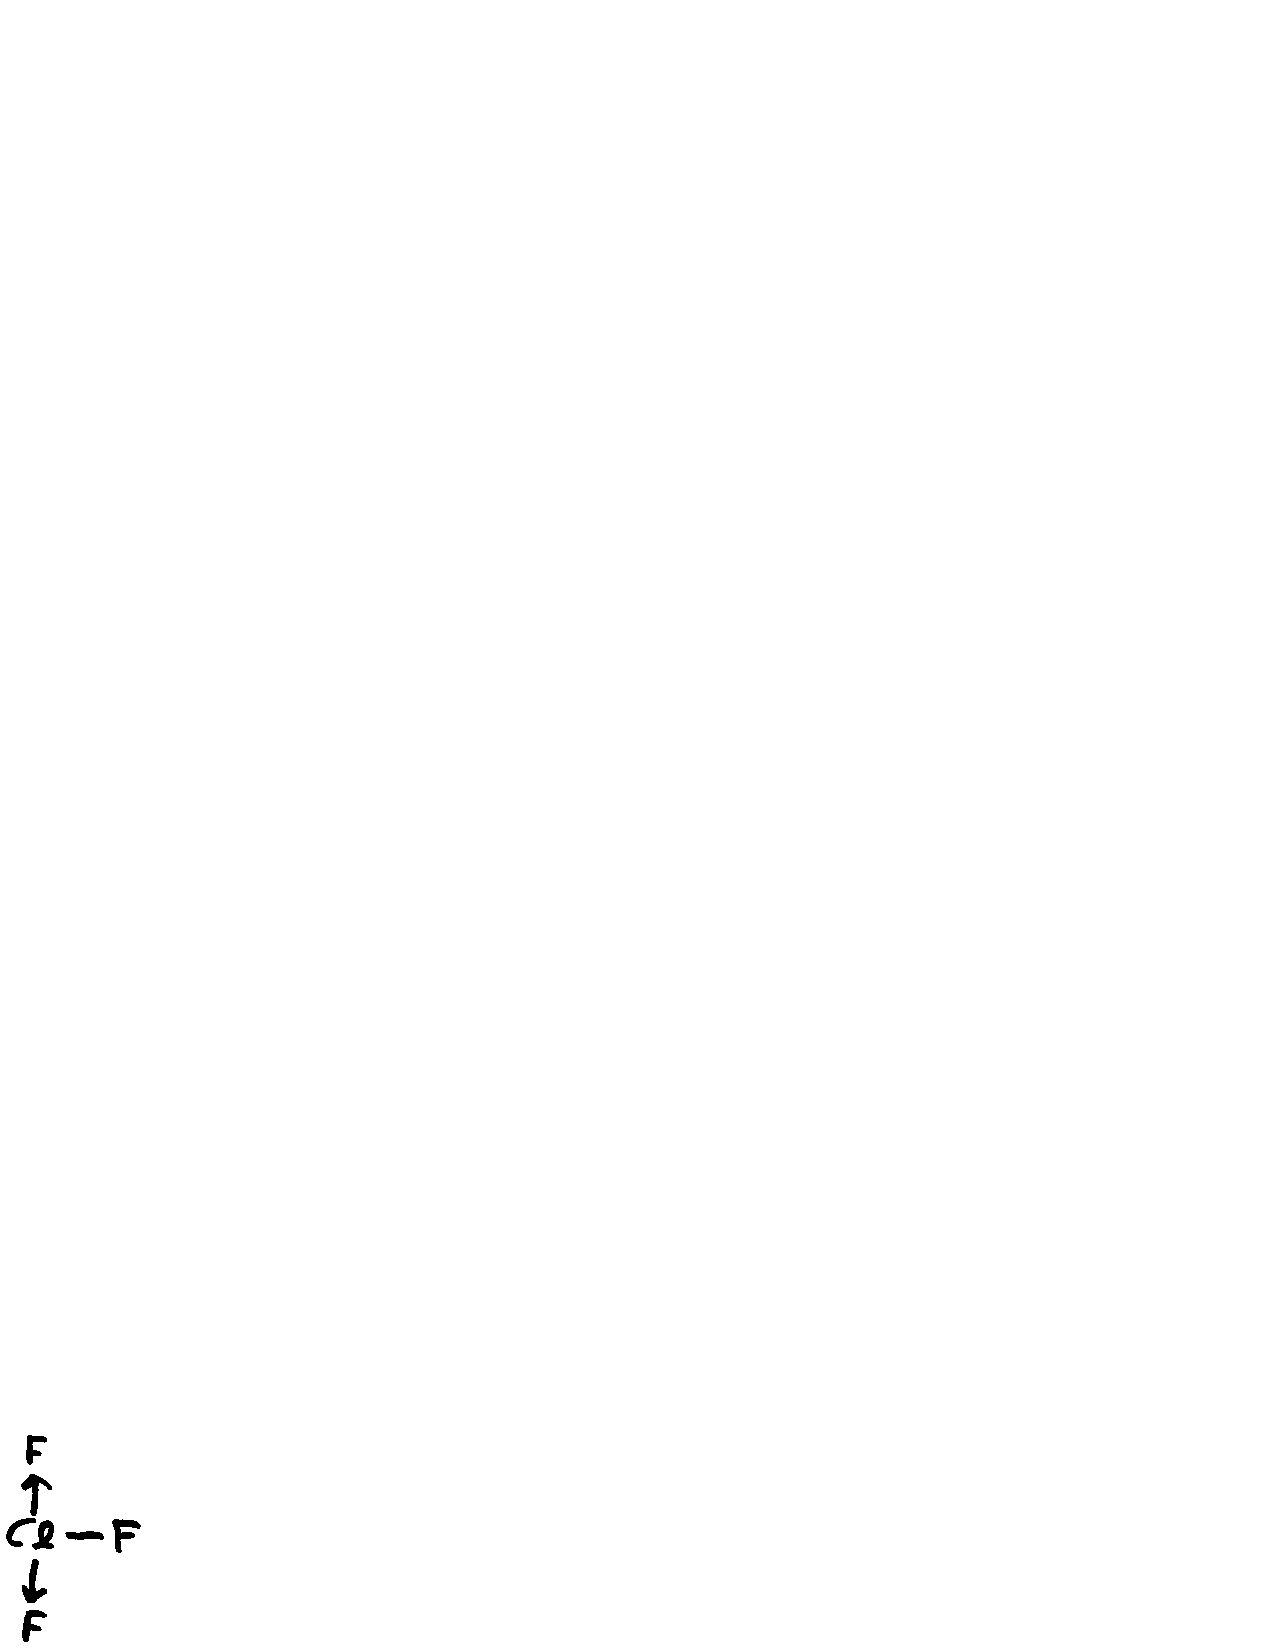
\includegraphics{fg11-f}
\label{chap11-eqno9}
\end{equation}
to be stable by 2.8 eV with respect to CIF + F + F.  Indeed, CIF$_3$ has been 
made and characterized.  The experimental value for the above bond energy 
is 2.6 eV rather than 2.8 eV, and the geometry is
\begin{equation}
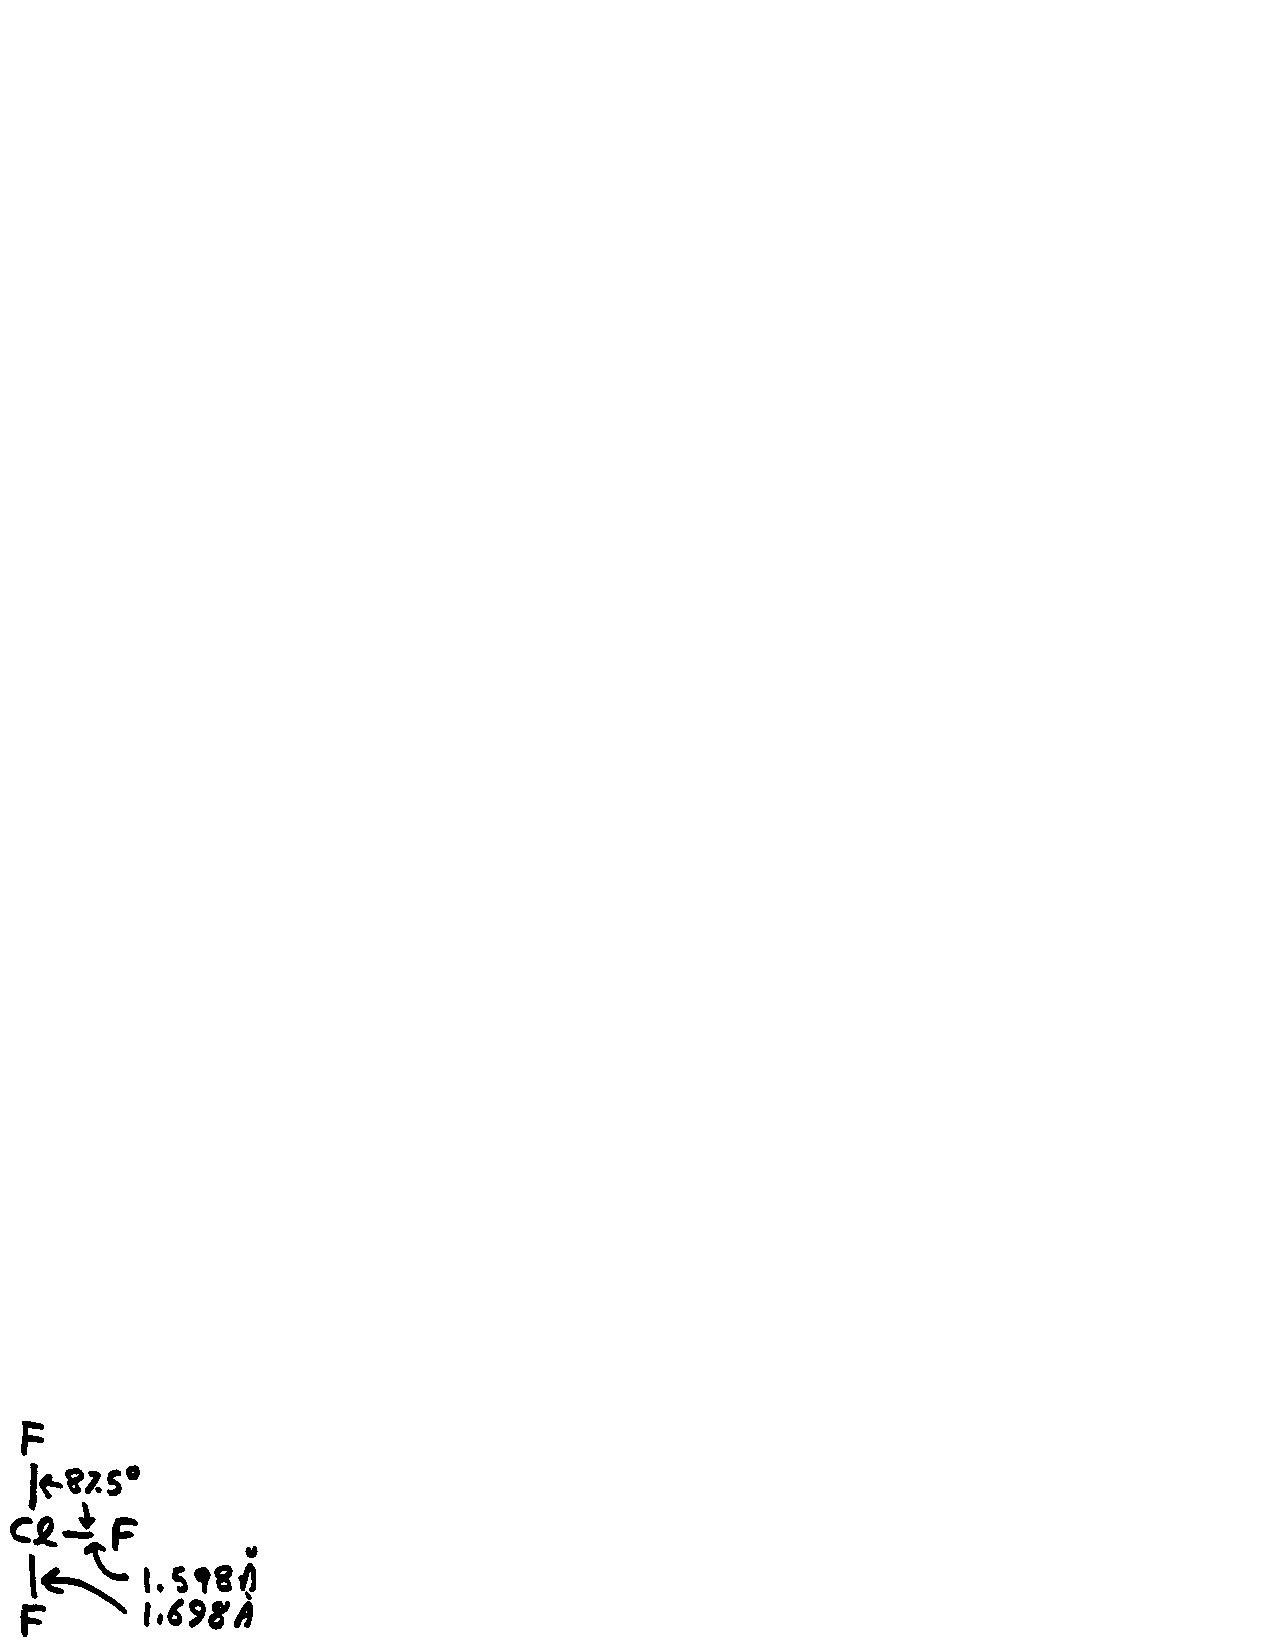
\includegraphics{fg11-g}
\label{chap11-eqno10}
\end{equation}

As expected, the F-Cl-F three-center, four-electron bond is nearly 
linear, bond angle 175$^{\circ}$. The reason why this angle is not linear 
has to do with the nonbonded interactions with the central ClF.  The $3s$ 
lone pair on the Cl pooches out the back side as the ClF sigma bond is formed
\begin{equation}
% missing figure from ch11 p 5 :cl-f:
%\includegraphics{fg11-??}
\label{chap11-eqno11}
\end{equation}

As the two new F atoms bond to the Cl to form the three-center bond, the F 
$p \sigma$ orbitals overlap the Cl $3s$ pair.  In order to avoid this 
problem, the two new F's rotate toward the center F slightly,

Our estimates in Table \ref{chap11-tab3} suggest that
\begin{equation}
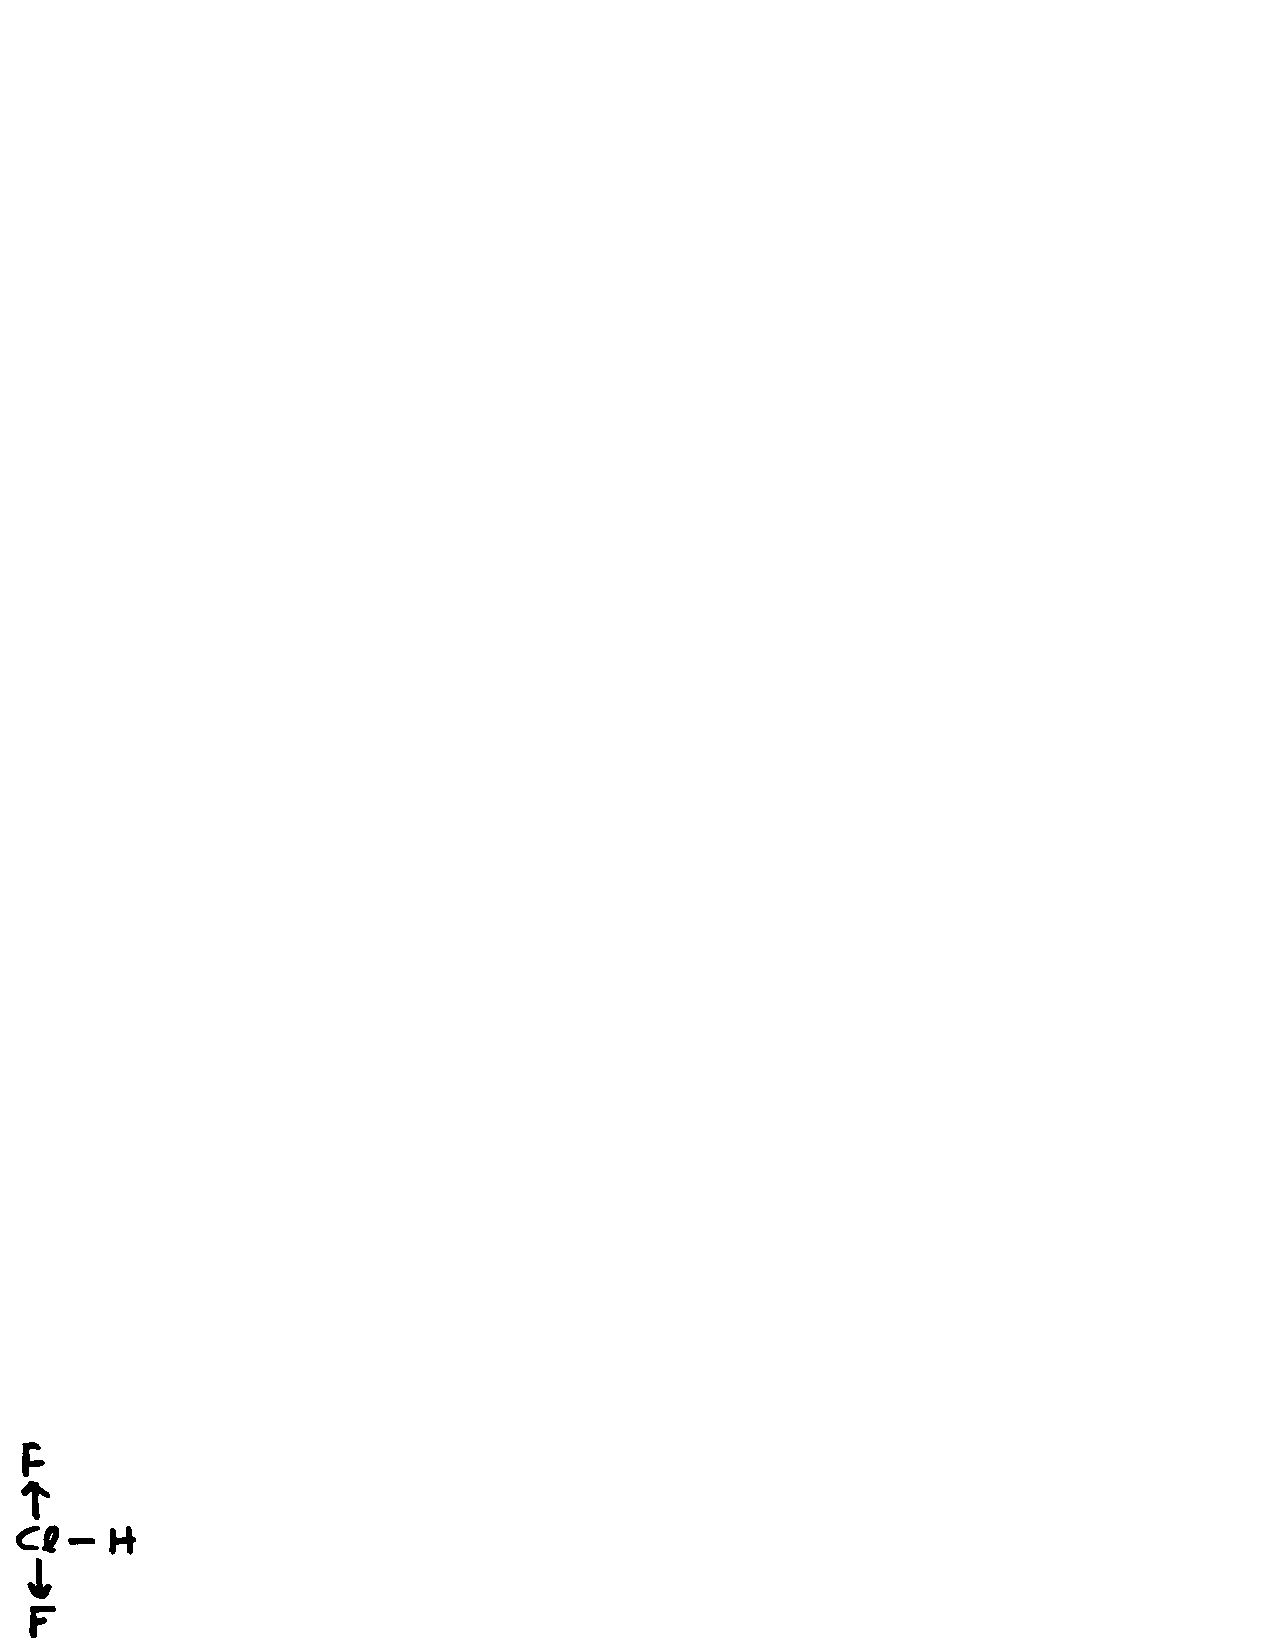
\includegraphics{fg11-h}
\label{chap11-eqno12}
\end{equation}
would also be quite stable, $\sim$2.7 eV for the three-center bond. The problem 
with this species is that it can decompose to
\begin{equation}
F_2 ClH \longrightarrow ClF + HF
\end{equation}
which, because of the very strong HF bond, is exothermic by 1.4 eV, 
using $D(HF) = 5.87$, $D(HCl) = 4.43$, and $D(ClF) = 2.62$ eV.  
As will be discussed in Chemistry 1c, the fact that a process is 
exothermic does not mean that it will proceed spontaneously.  To do 
so requires a process by which bonds can be broken and formed in a 
sequence, mechanism, that avoids a high energy step.
However, there is likely to be such a mechanism for this species. 

\subsection{ClF$_5$}

The ClF$_3$ molecule equation (\ref{chap11-eqno9}) has an additional
doubly-occupied $p$ orbital not yet used for bonding.  Thus, ClF$_5$
is expected to be strongly bound and to have the geometry
\begin{equation}
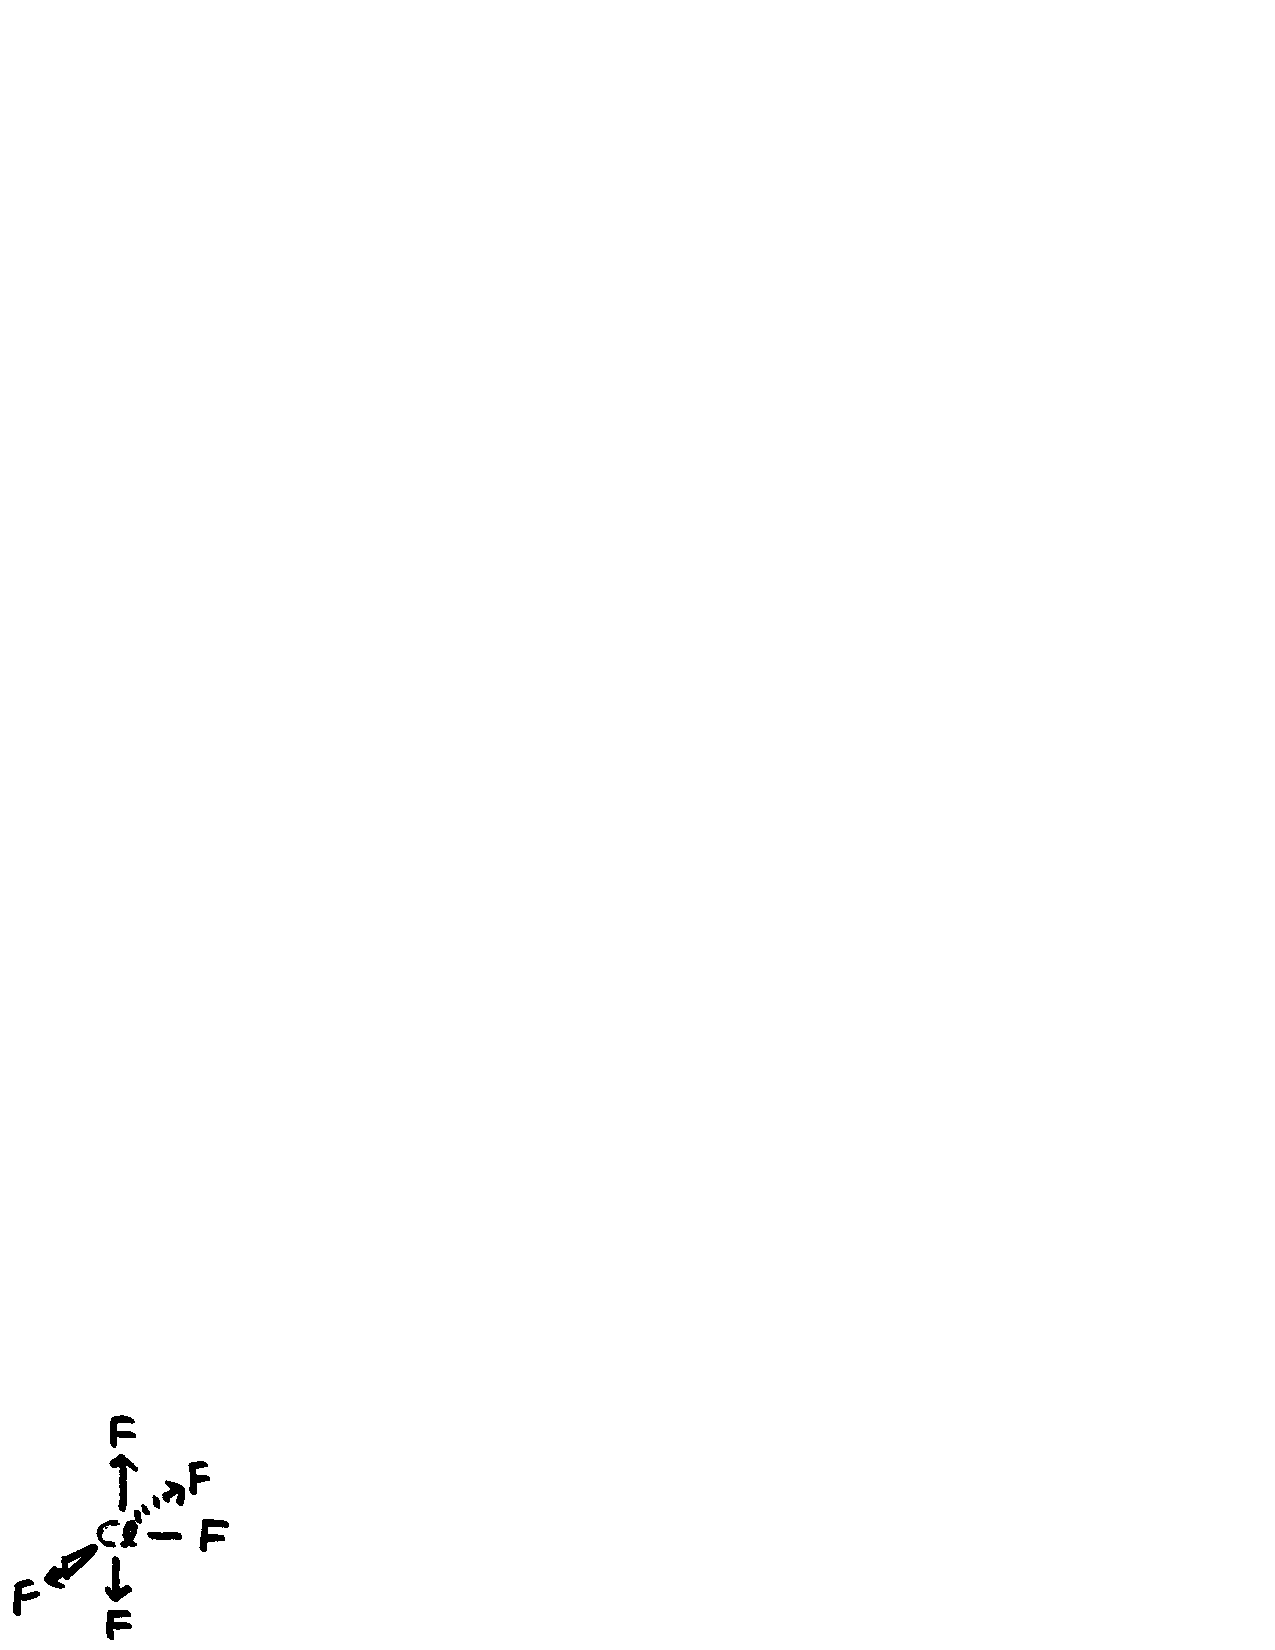
\includegraphics{fg11-i}
\label{chap11-eqno13}
\end{equation}
of a square pyramid with the four equatorial F{\it s} involved on the two 
three-electron sigma bonds, nearly in the same plane as the Cl. Indeed, 
this is the case with F$_{eq}$ClF$_{ax}$ angle being 86.5$^{\circ}$.

We have now used up the three Cl $p$ orbitals and hence, correctly do not 
expect any more F{\it s} to bond to the Cl.

Considering negative ions, Cl$^-$ is analogous to Xe but with a very low 
ionization potentiat, 3.6 eV.  Thus, ClF$^-_2$ and ClF$^-_4$ are expected 
to be linear and square planar, respectively.  ClF$^-_6$ is not stable.

\subsection{BrF$_n$, IF$_n$}

Br forms BrF$_3$ and BrF$_5$ compounds analogous to ClF$_3$ and BrF$_3$ 
with similar structure.  In addition to BrF$^-_2$ and BrF$^-_4$, 
Br$^-$ also forms a stable BrF$^-_6$.

I forms all the above compounds observed for Br, but also forms 
IF$_7$.  Clearly, the bonding is more complicated for IF$_7$.

\section{SF$_n$}

SF$_2$ has the structure
\begin{equation}
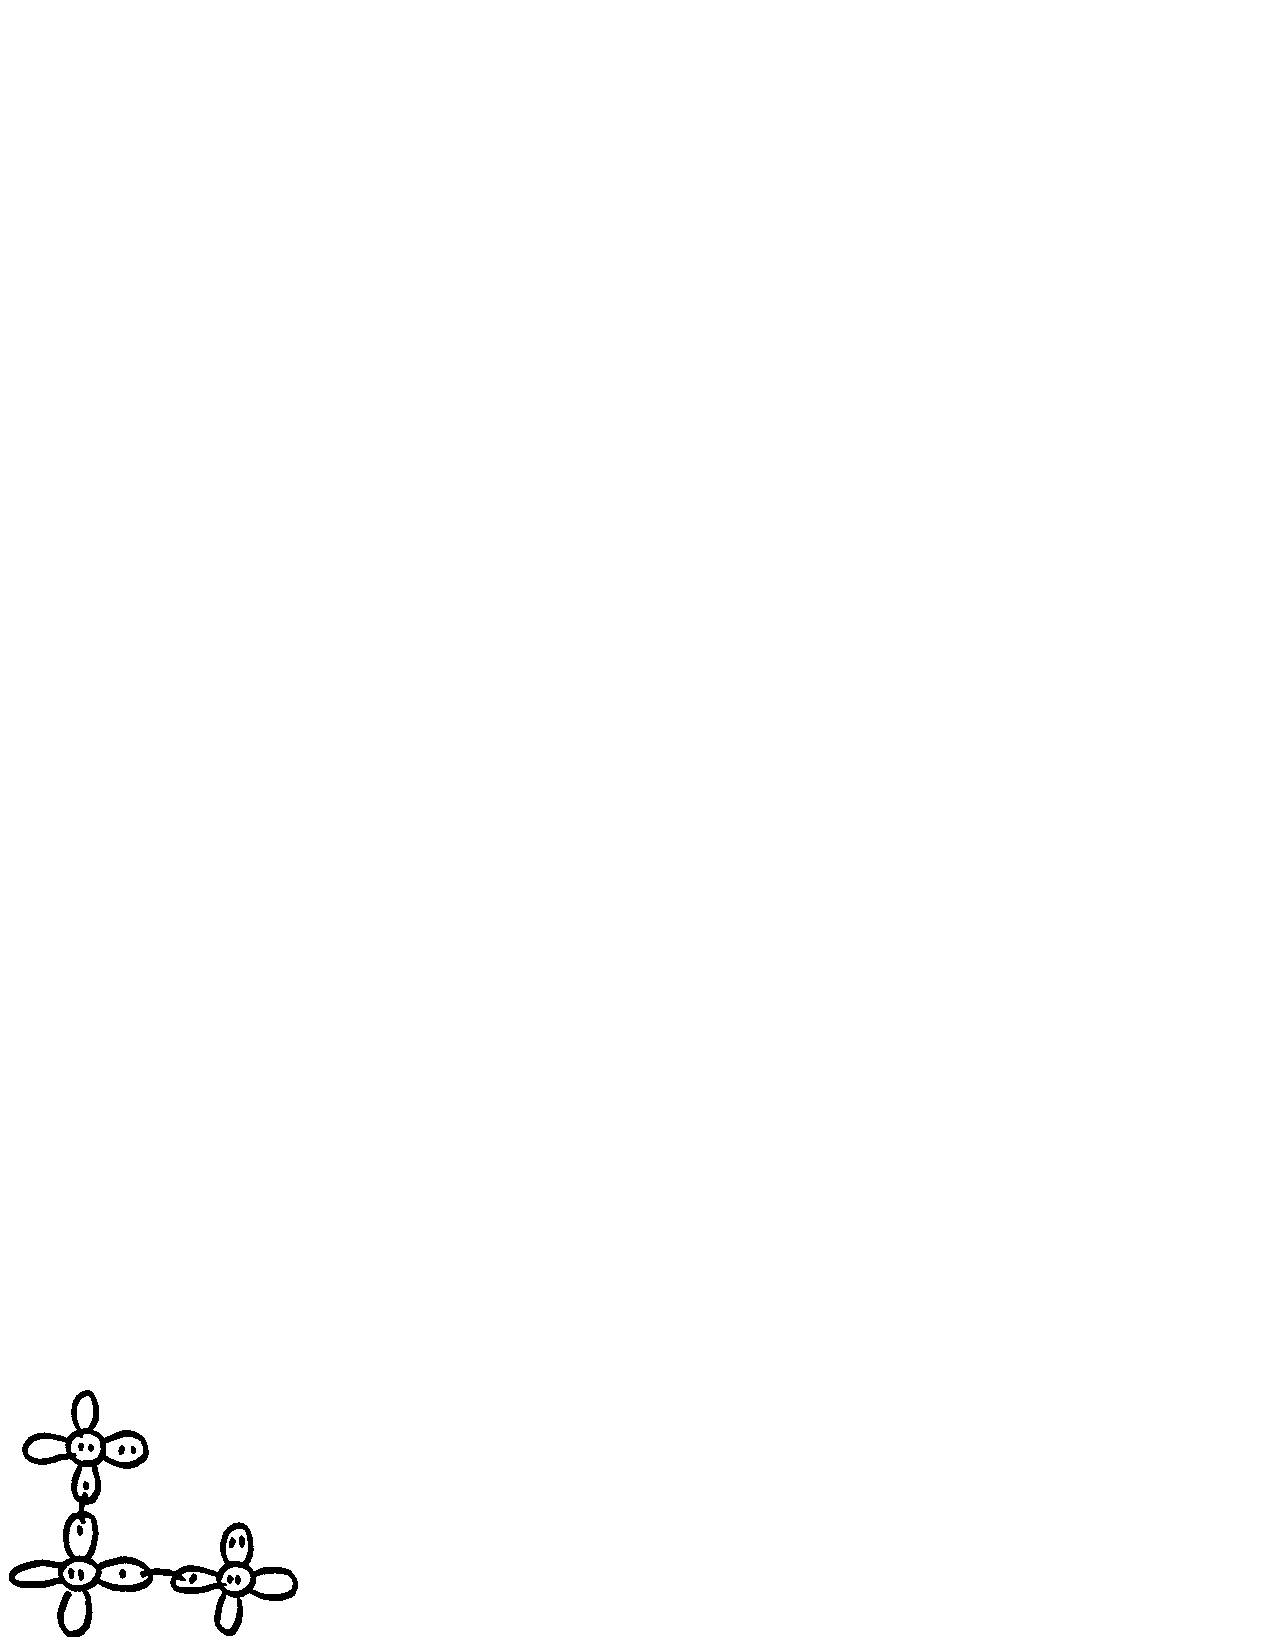
\includegraphics{fg11-j}
\end{equation}
leading to an FSF bond angle of 102$^{\circ}$.  Thus, there is a $p$ 
pair available for making a three-center sigma bond to two fluorines. 
Indeed, SF$_4$ has the expected structure
\begin{equation}
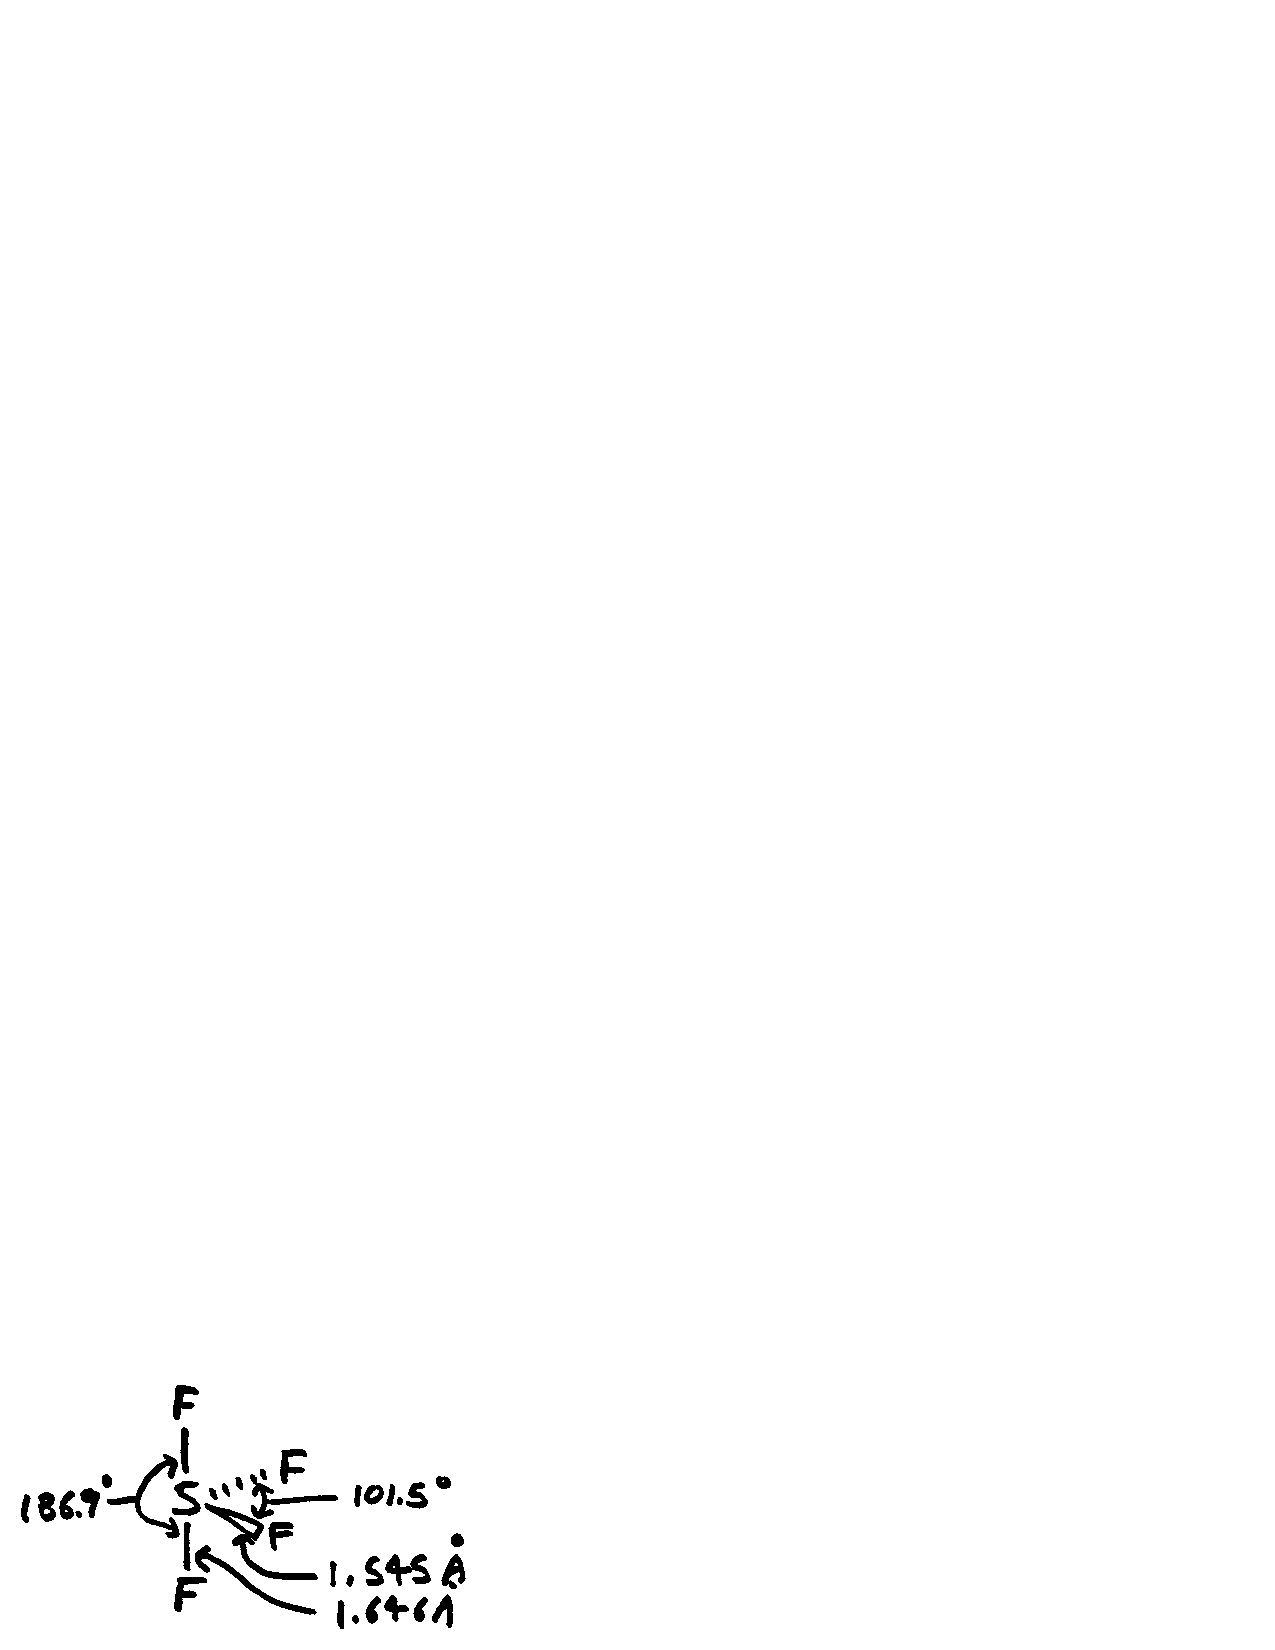
\includegraphics{fg11-k}
\end{equation}
where the S $3s$ pair pooches to the left.

On the other hand, SF$_6$ has an octahedral geometry
\begin{equation}
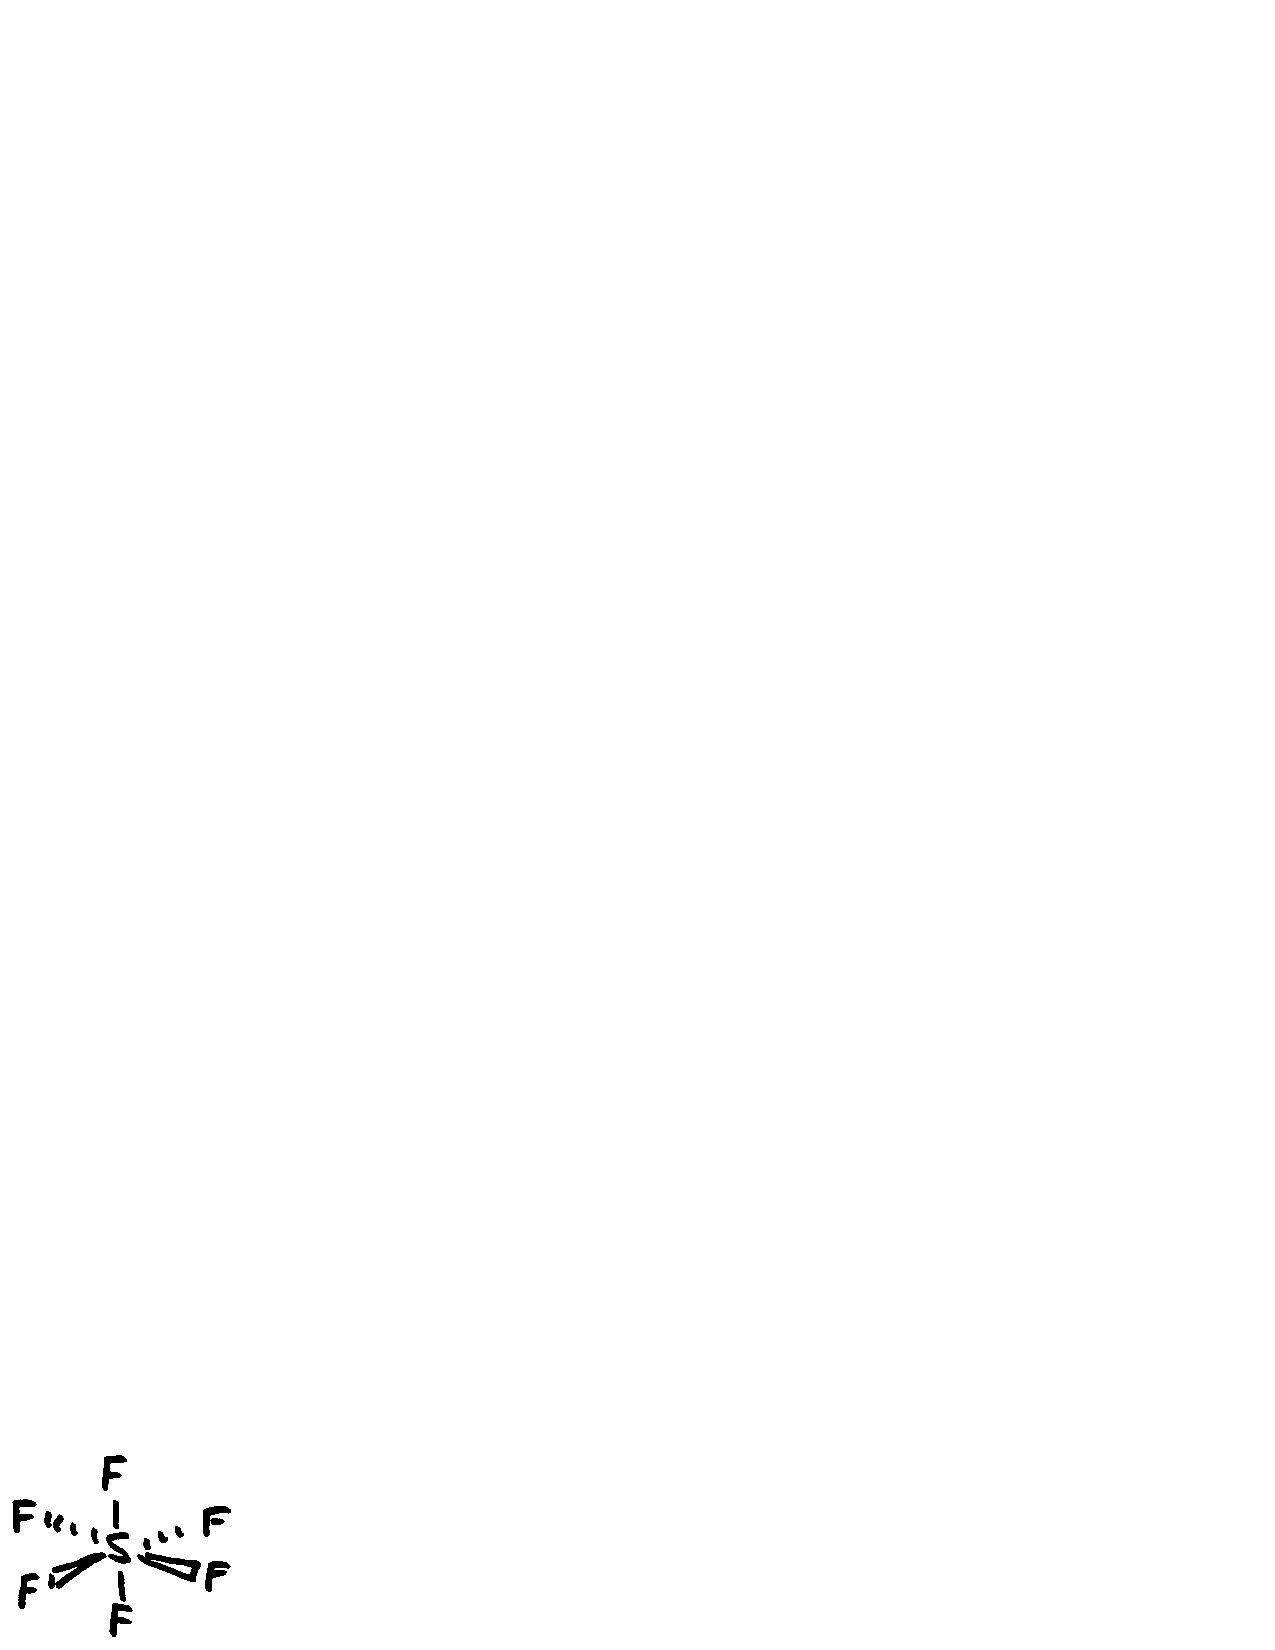
\includegraphics{fg11-l}
\end{equation}
with six equivalent bonds.  Sometimes this structure is rationalized in 
terms of $sp^3d^2$ hybrid orbitals.  However, calculations do not find 
such a large amount of $d$ character in the orbitals.

\section{PF$_n$}

PF$_3$ and PCl$_3$ have pyramidal geometries with bond angles of 
102$^{\circ}$.  However, PF$_5$ is also stable, and leads to a trigonal 
bipyramidal geometry,
\begin{equation}
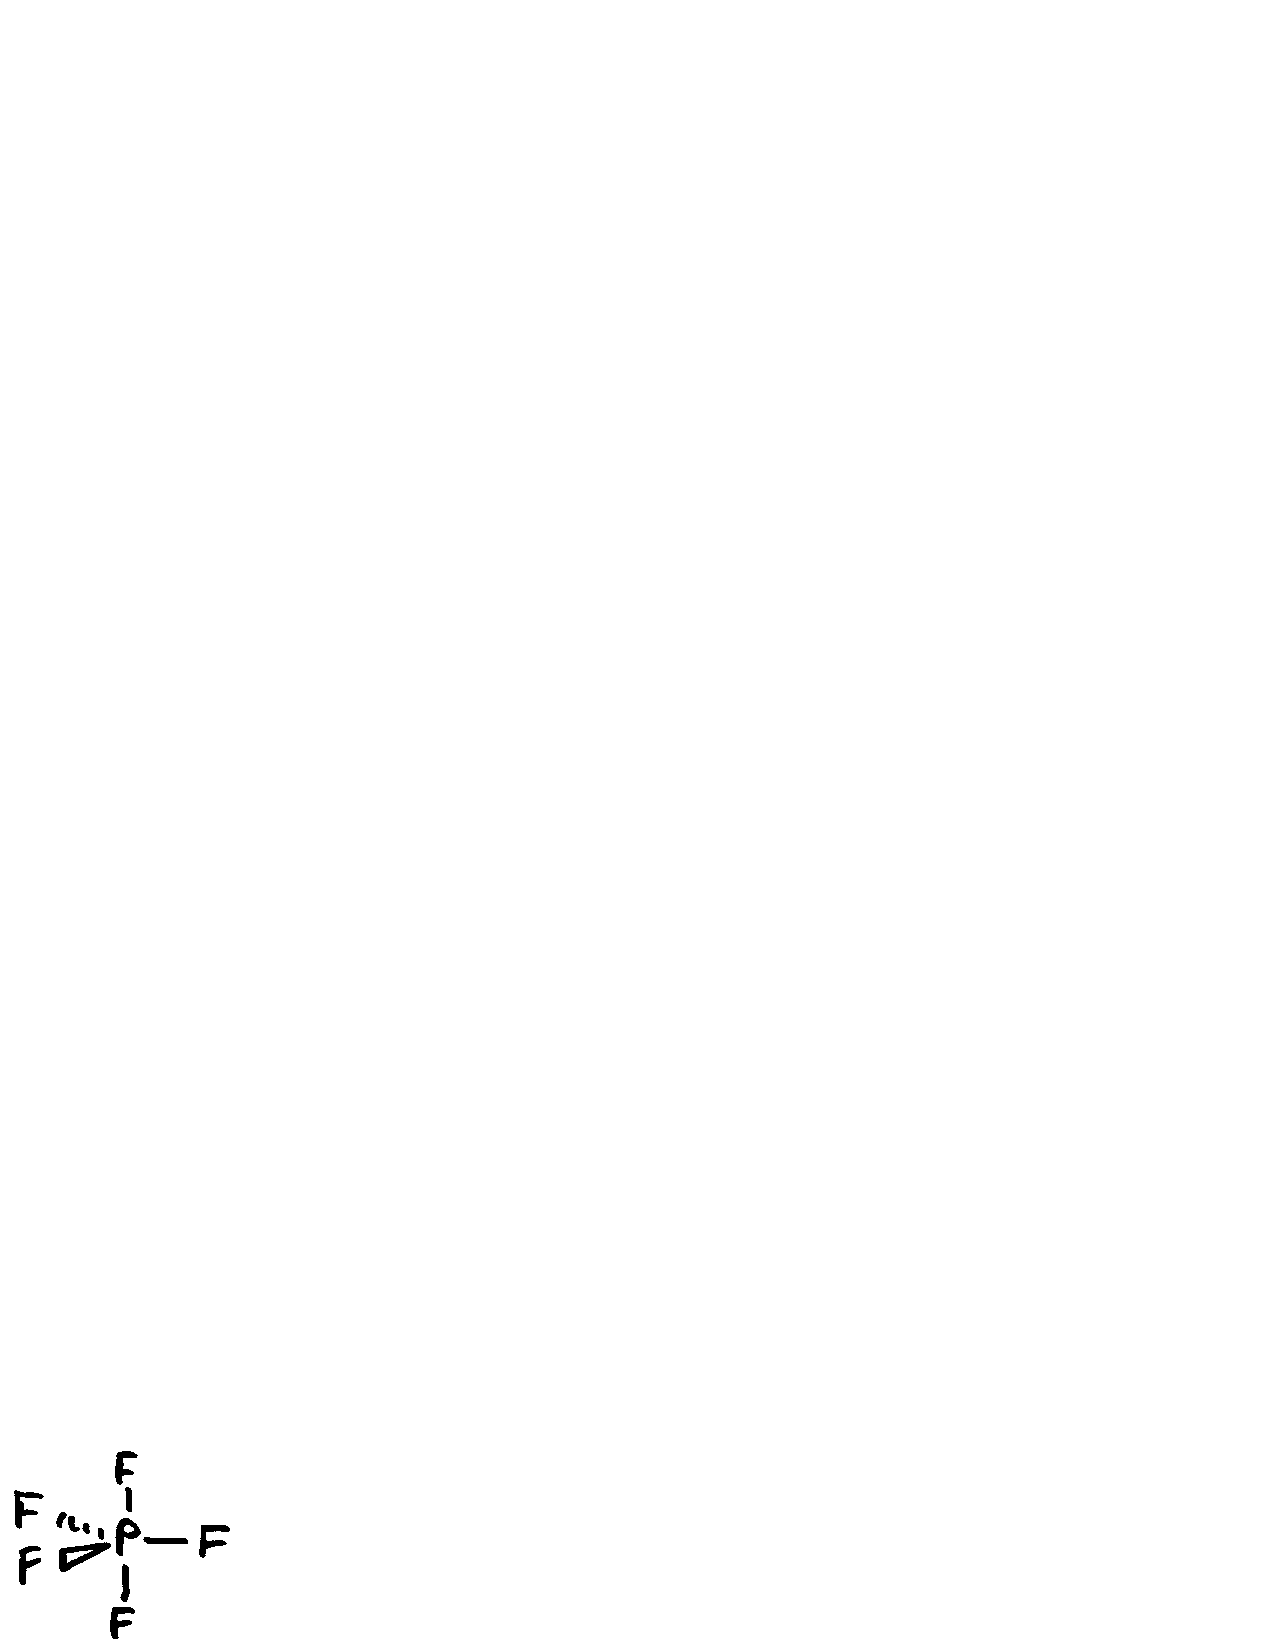
\includegraphics{fg11-m}
\end{equation}

\section{Donor-Acceptor Bonds to Oxygen}

PCl$_3$ forms a very strong bond to oxygen that can be viewed as bonding the P 
lone pair to the excited form of oxygen, having two doubly-occupied $p$ 
orbitals and one empty orbital
\begin{equation}
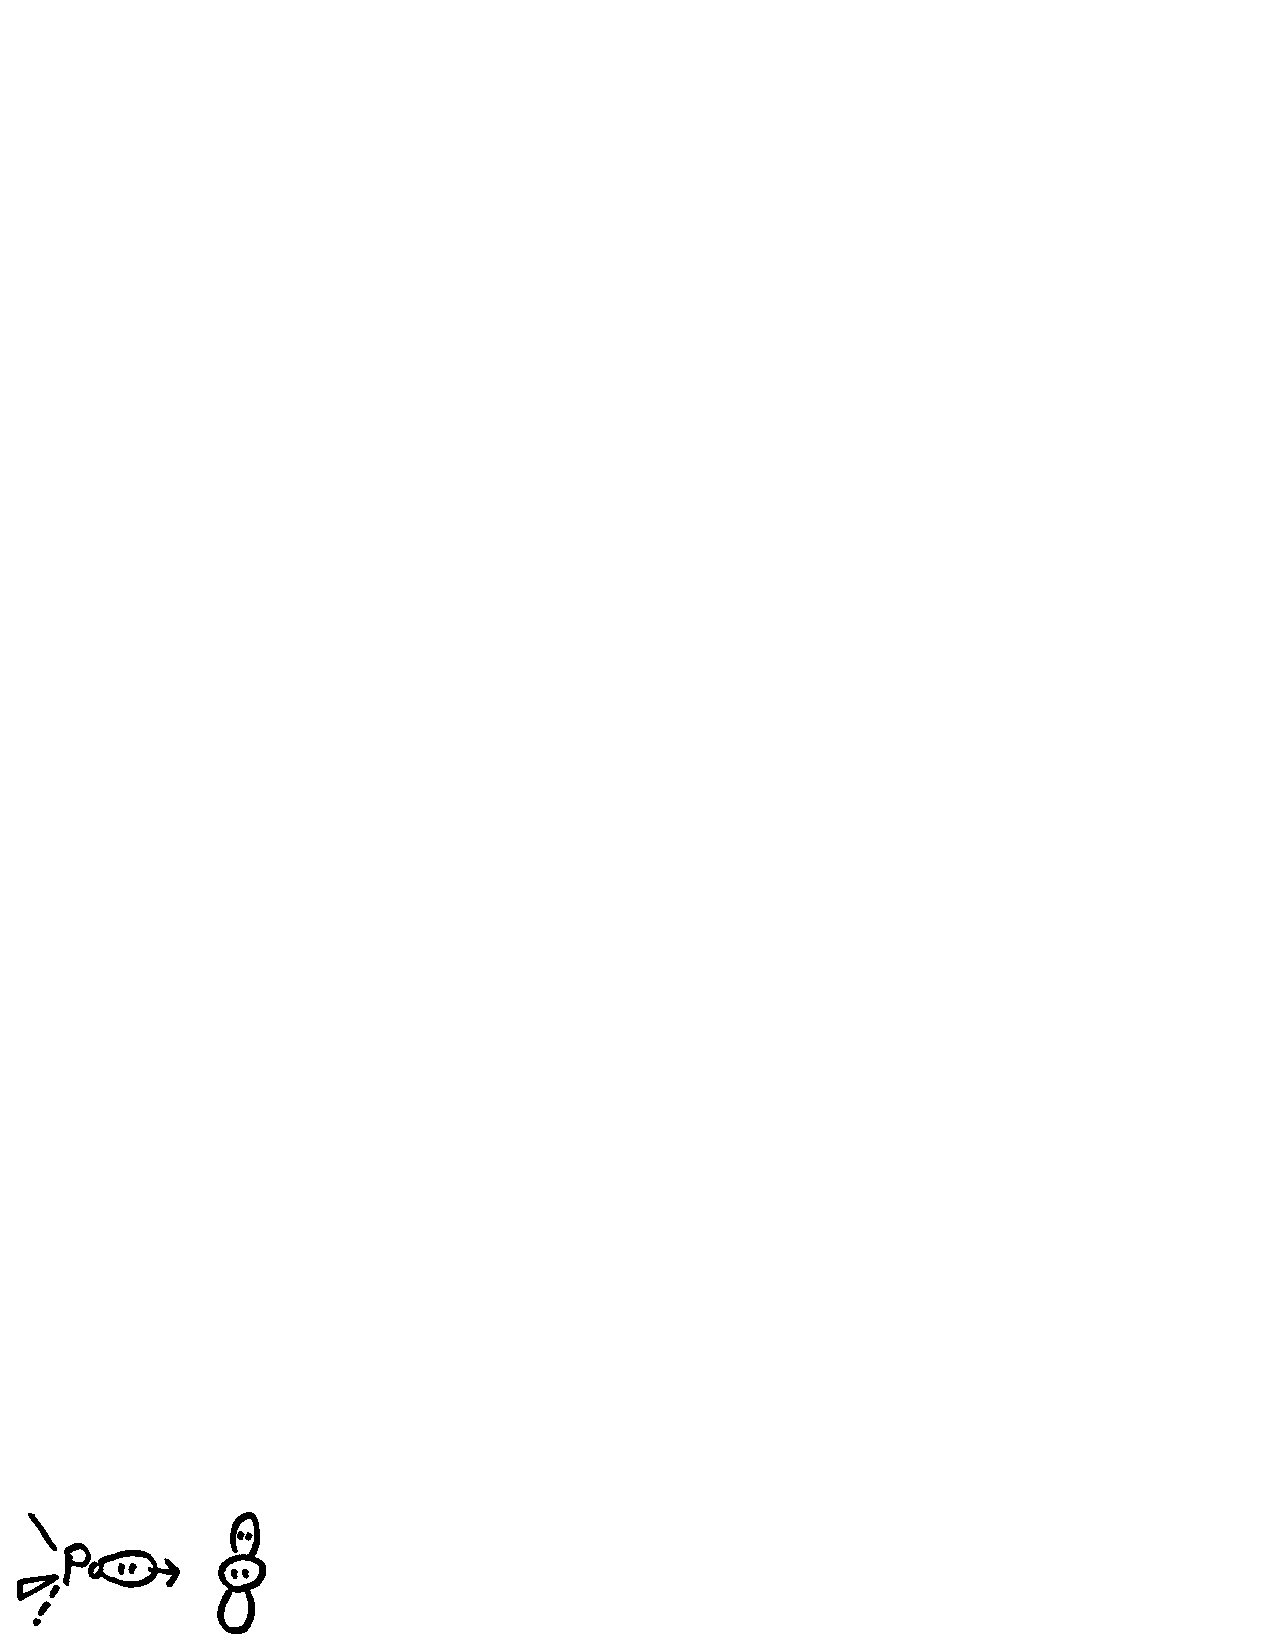
\includegraphics{fg11-n}
\end{equation}
There is a lot of charge transfer toward the oxygen so that one might also 
view this in terms of charge transfer
\begin{equation}
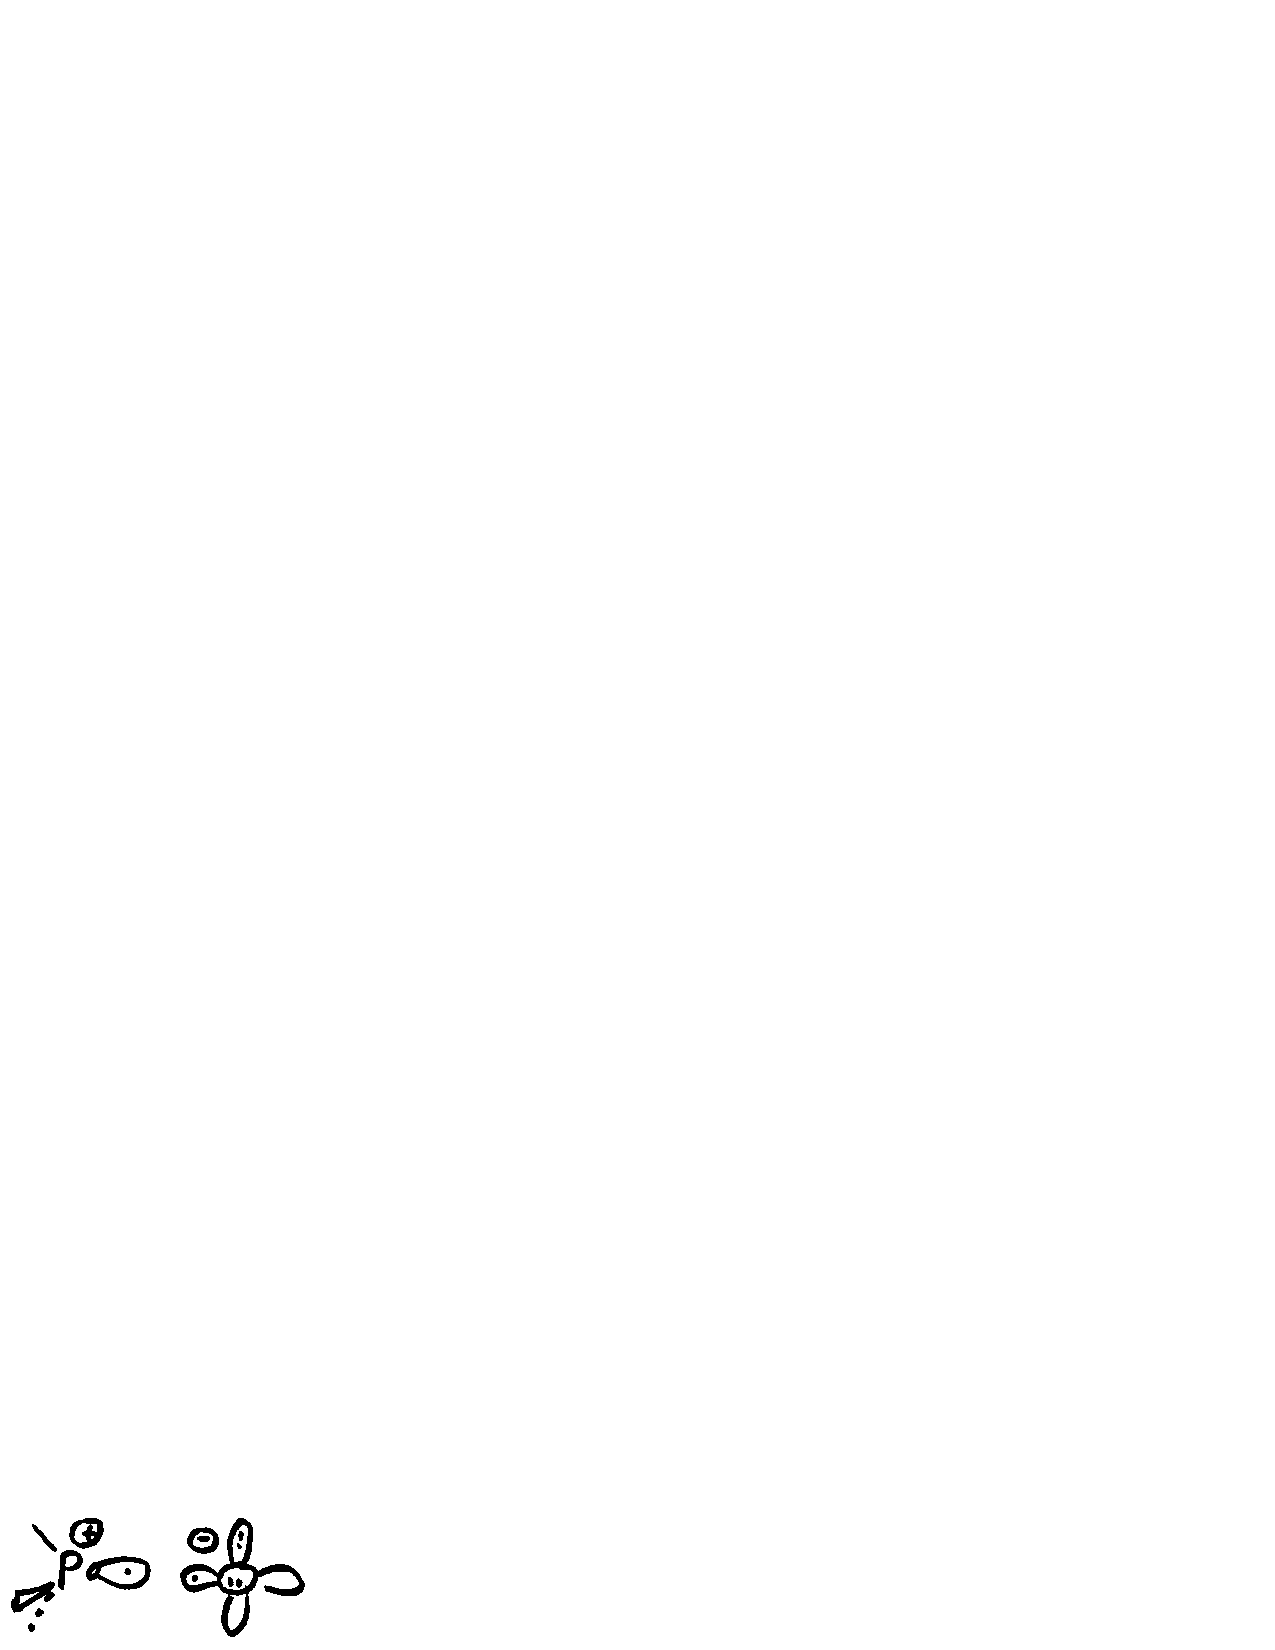
\includegraphics{fg11-o}
\end{equation}

\section{Ozone}

The molecular orbital description of O$_2$ is
\begin{equation}
( 3 \sigma_g )^2 (1 \pi_u )^4 (1 \pi_g )^2
\end{equation}
ignoring the $1s$ and $2s$ derived orbitals, where there is one electron in 
$\pi_{gz}$ and one in $\pi_{gy}$, triplet-coupled.  The valence bond 
description is
\begin{equation}
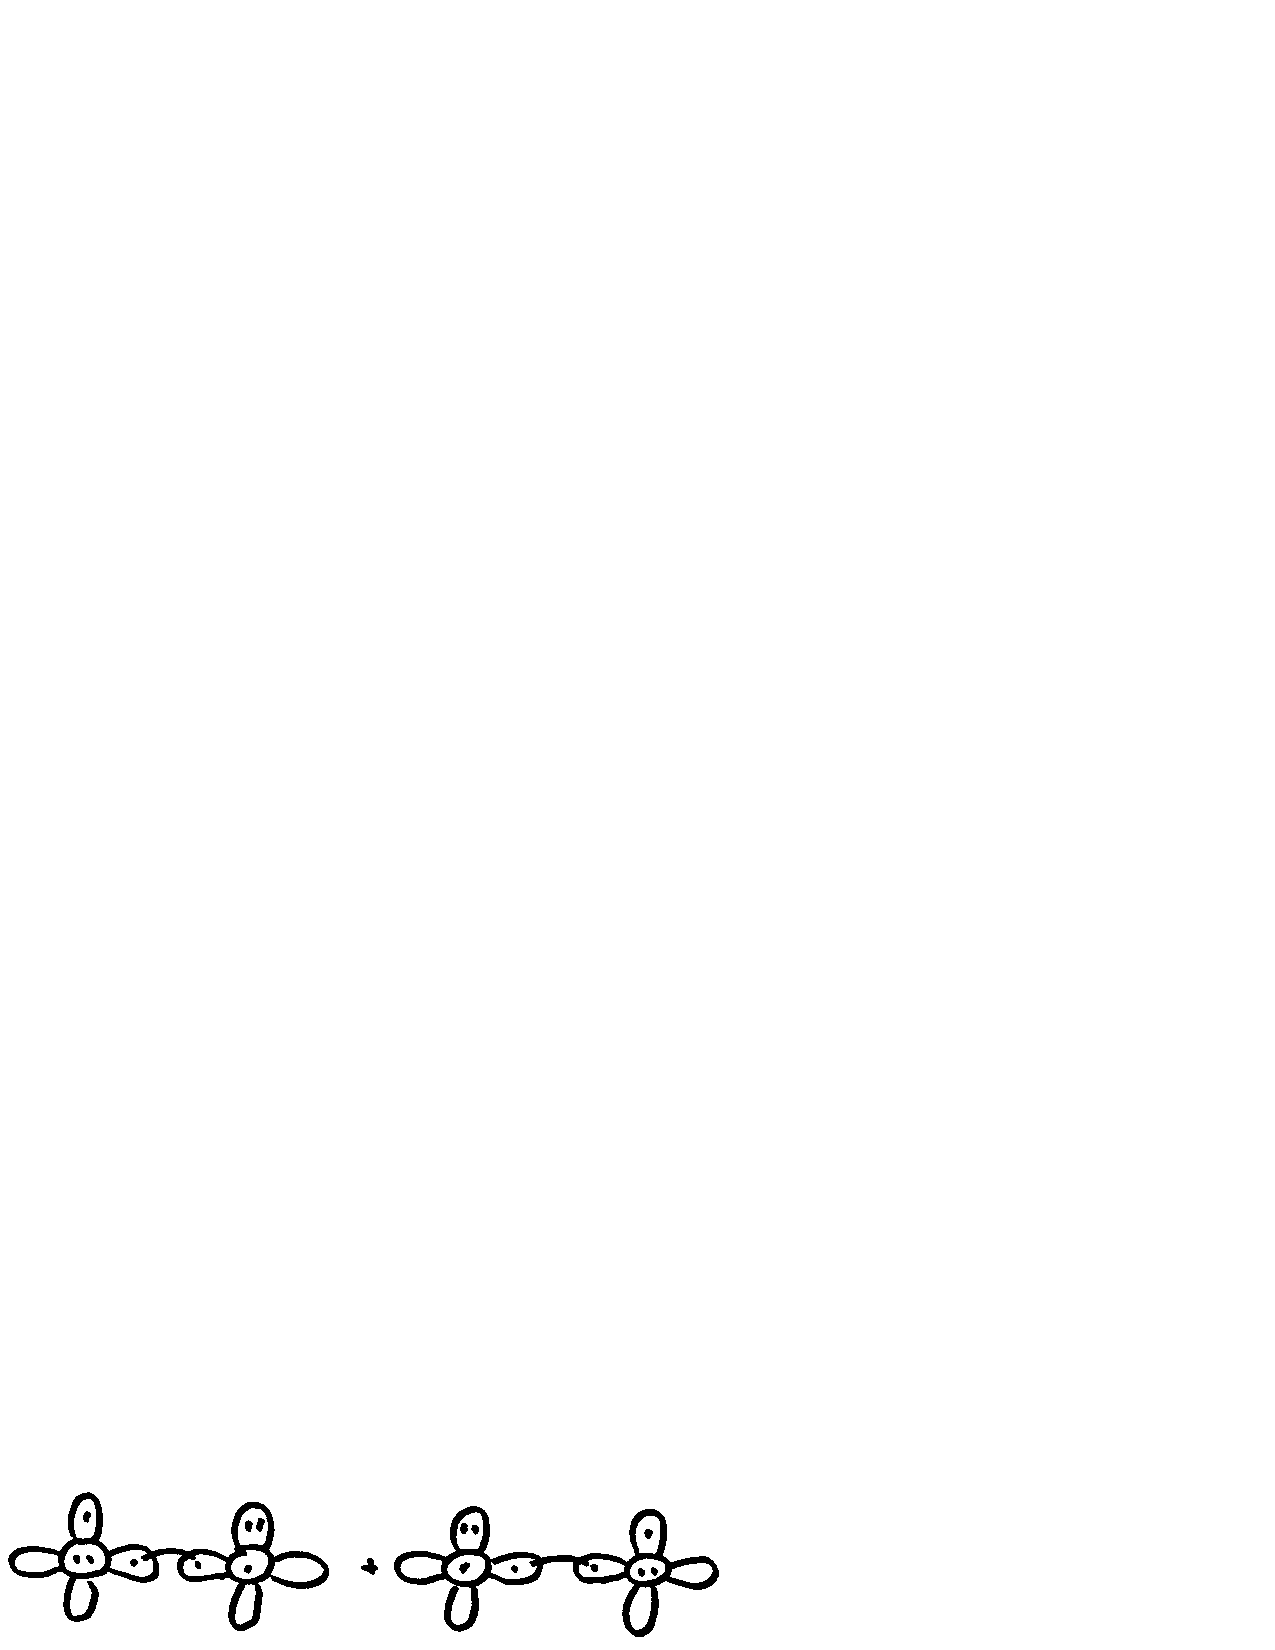
\includegraphics{fg11-p}
\end{equation}
with two three-electron bonds in each of the resonating configurations.

Bonding an H to O$_2$ leads to one dominant configuration,
\begin{equation}
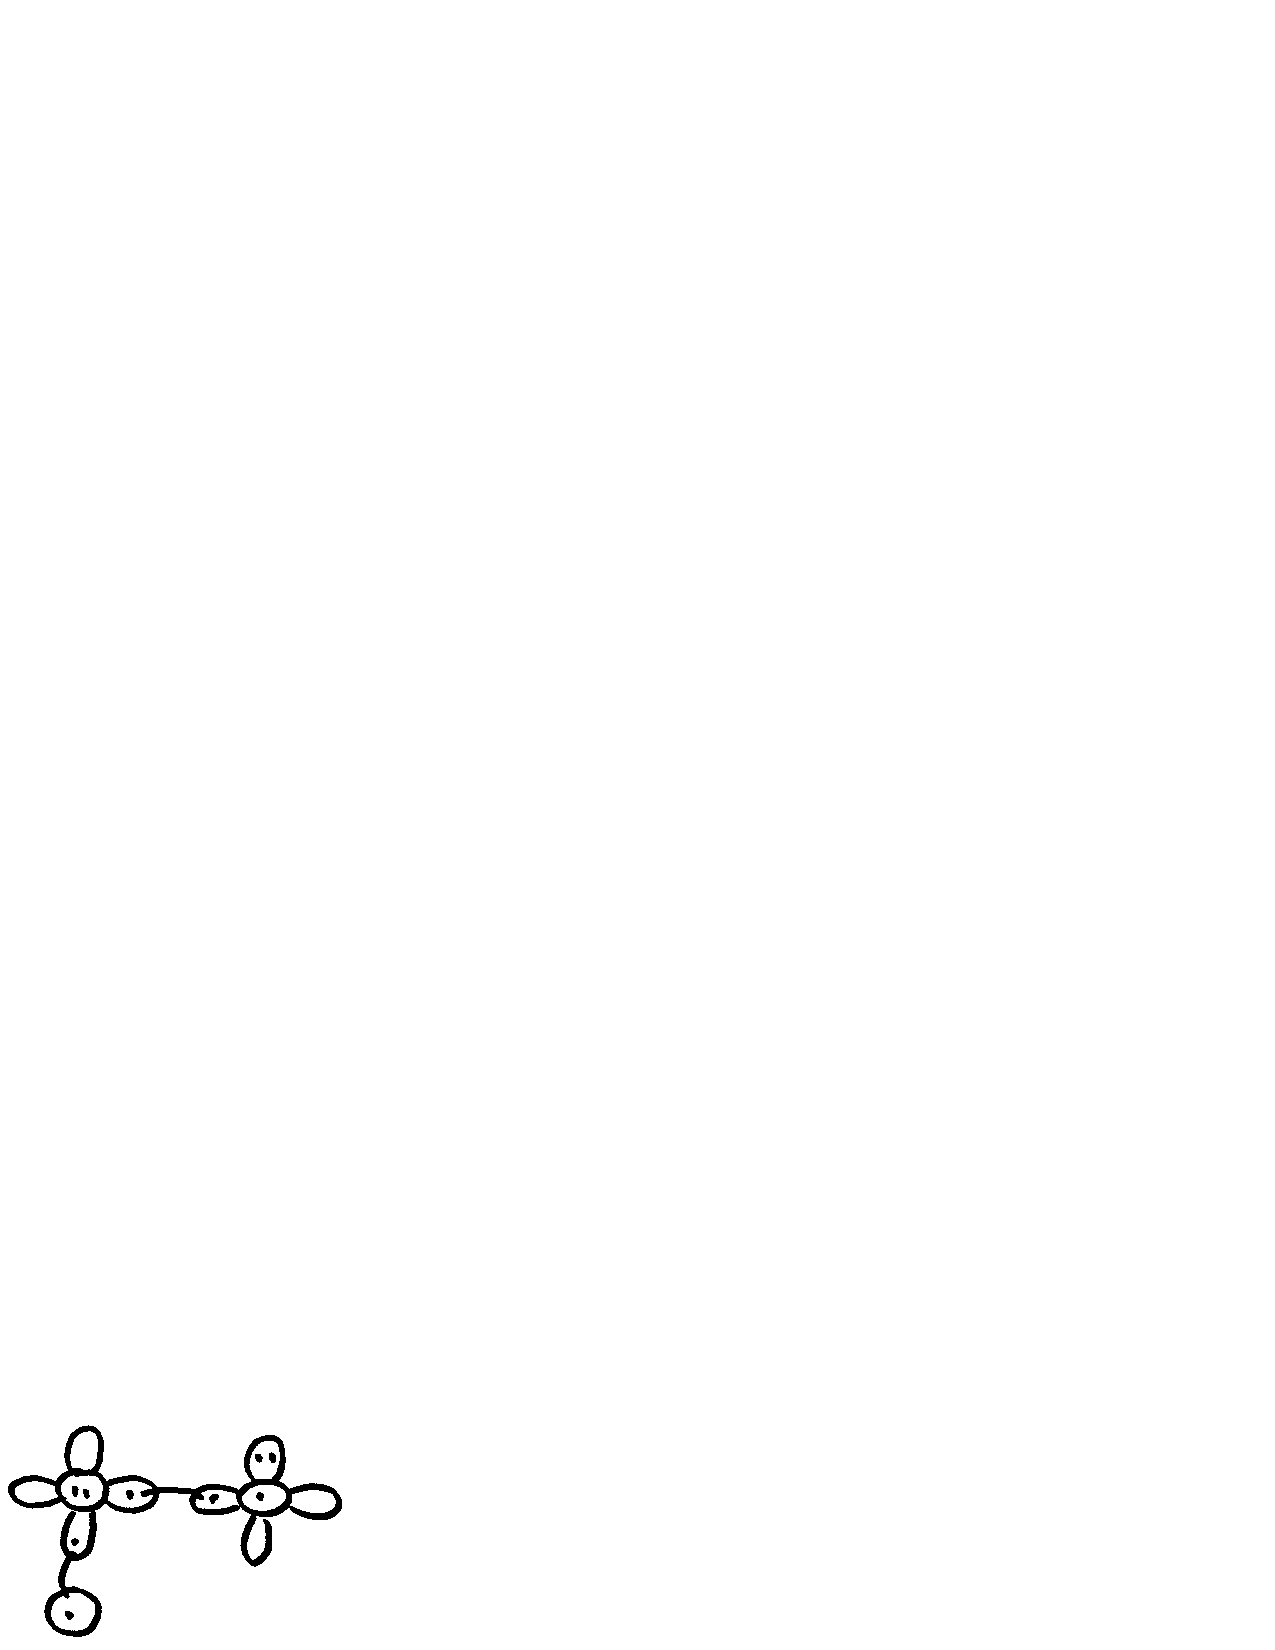
\includegraphics{fg11-q}
\end{equation}
However, there is still some three-electron bond character in the pi 
bond, perpendicular to the plane, leading to
\begin{equation}
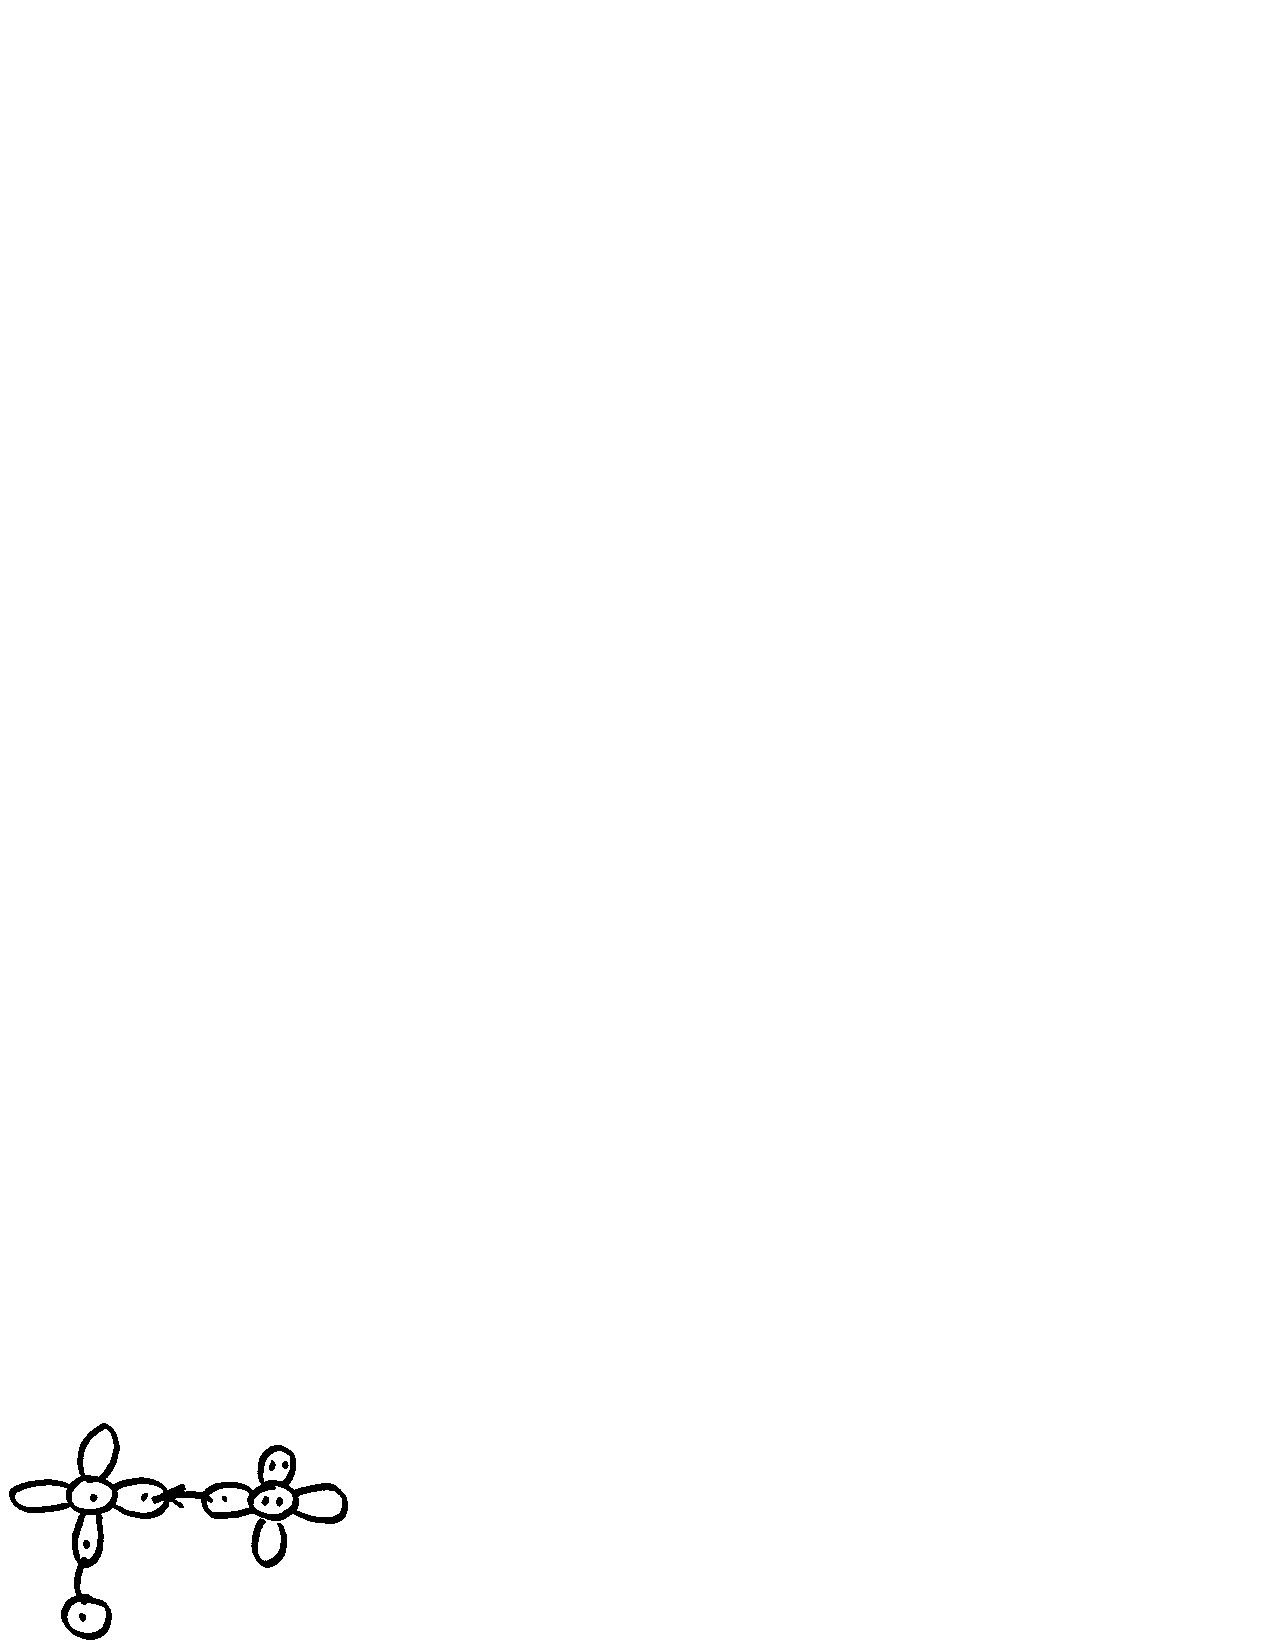
\includegraphics{fg11-r}
\end{equation}

Bonding a third O to O$_2$ to form ozone, O$_3$, we can consider two 
possibilities.  In order to form two bonds to each O, we could make the 
molecular triangle
\begin{equation}
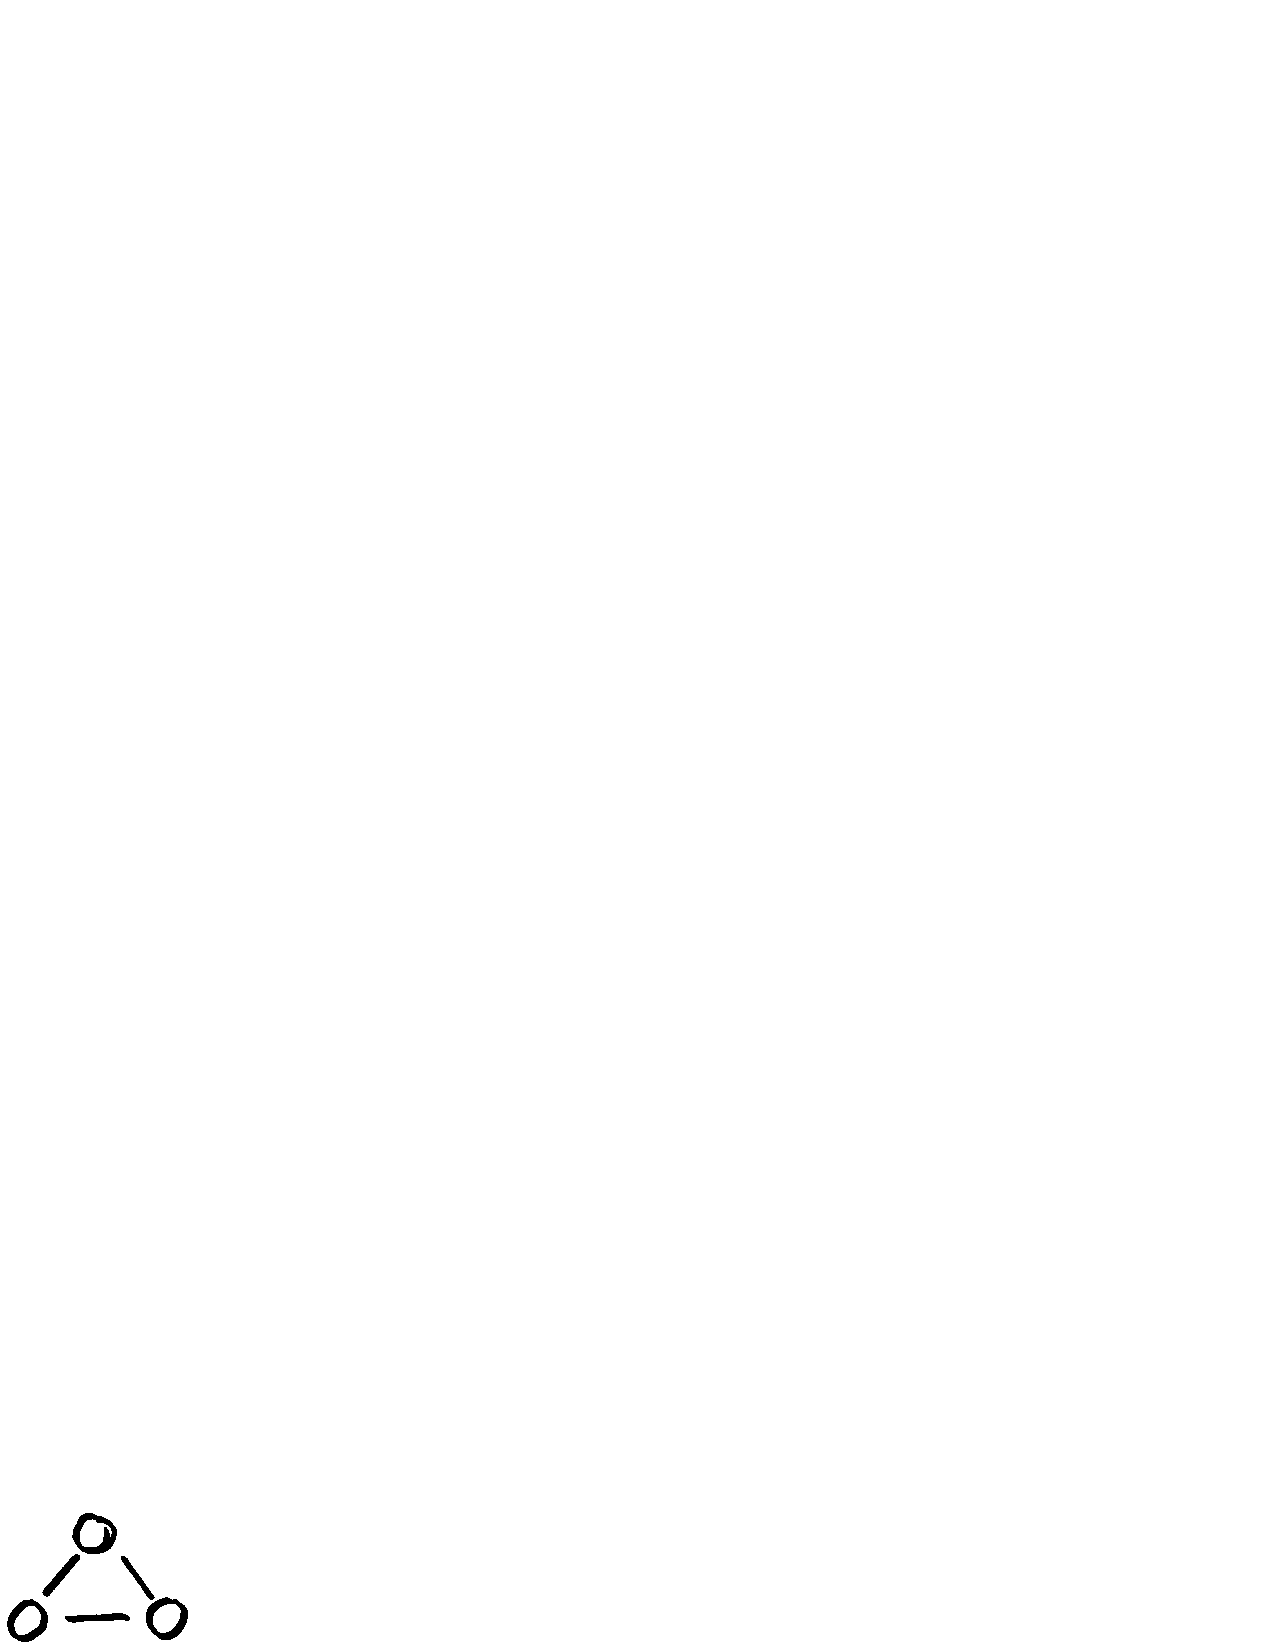
\includegraphics{fg11-s}
\end{equation}
However, the intrinsic O-O sigma bond energies, $\sim$48 kcal, and strain 
energy, $\sim$26 kcal due to the bad bond angle, are such that this 
species should have about the same energy as O$_2 +$ O.  The bond energy 
of O$_2$ is 118 kcal; the predicted bond energy of ring O$_3$ 
is $3 \times 48 - 26 = 118$ kcal.

The other possibility is to bond the new O in the same way as the H, 
leading to
\begin{equation}
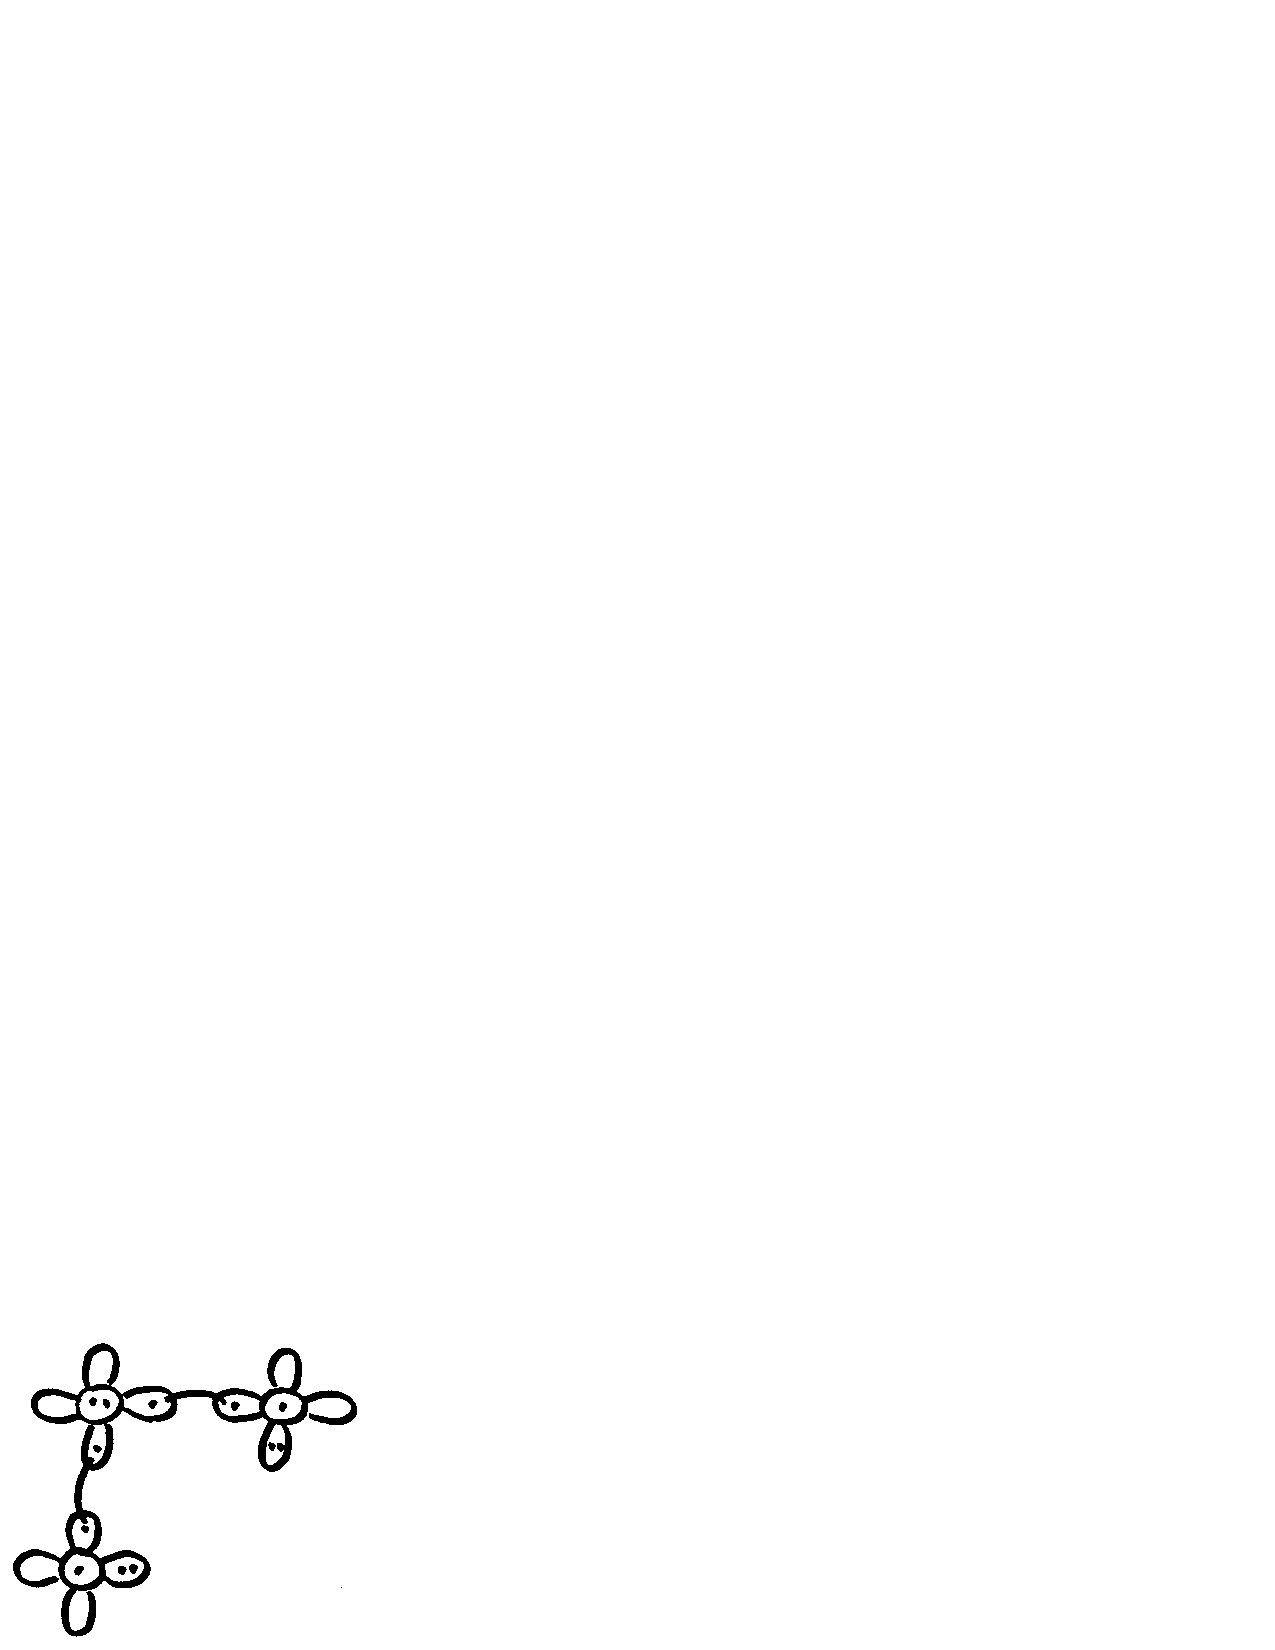
\includegraphics{fg11-t}
\end{equation}
Here the pi electrons on the terminal oxygens are not doing much. This is 
analogous to the sigma system in covalent XeF$_2$, and we should consider 
the charge transfer to obtain
\begin{equation}
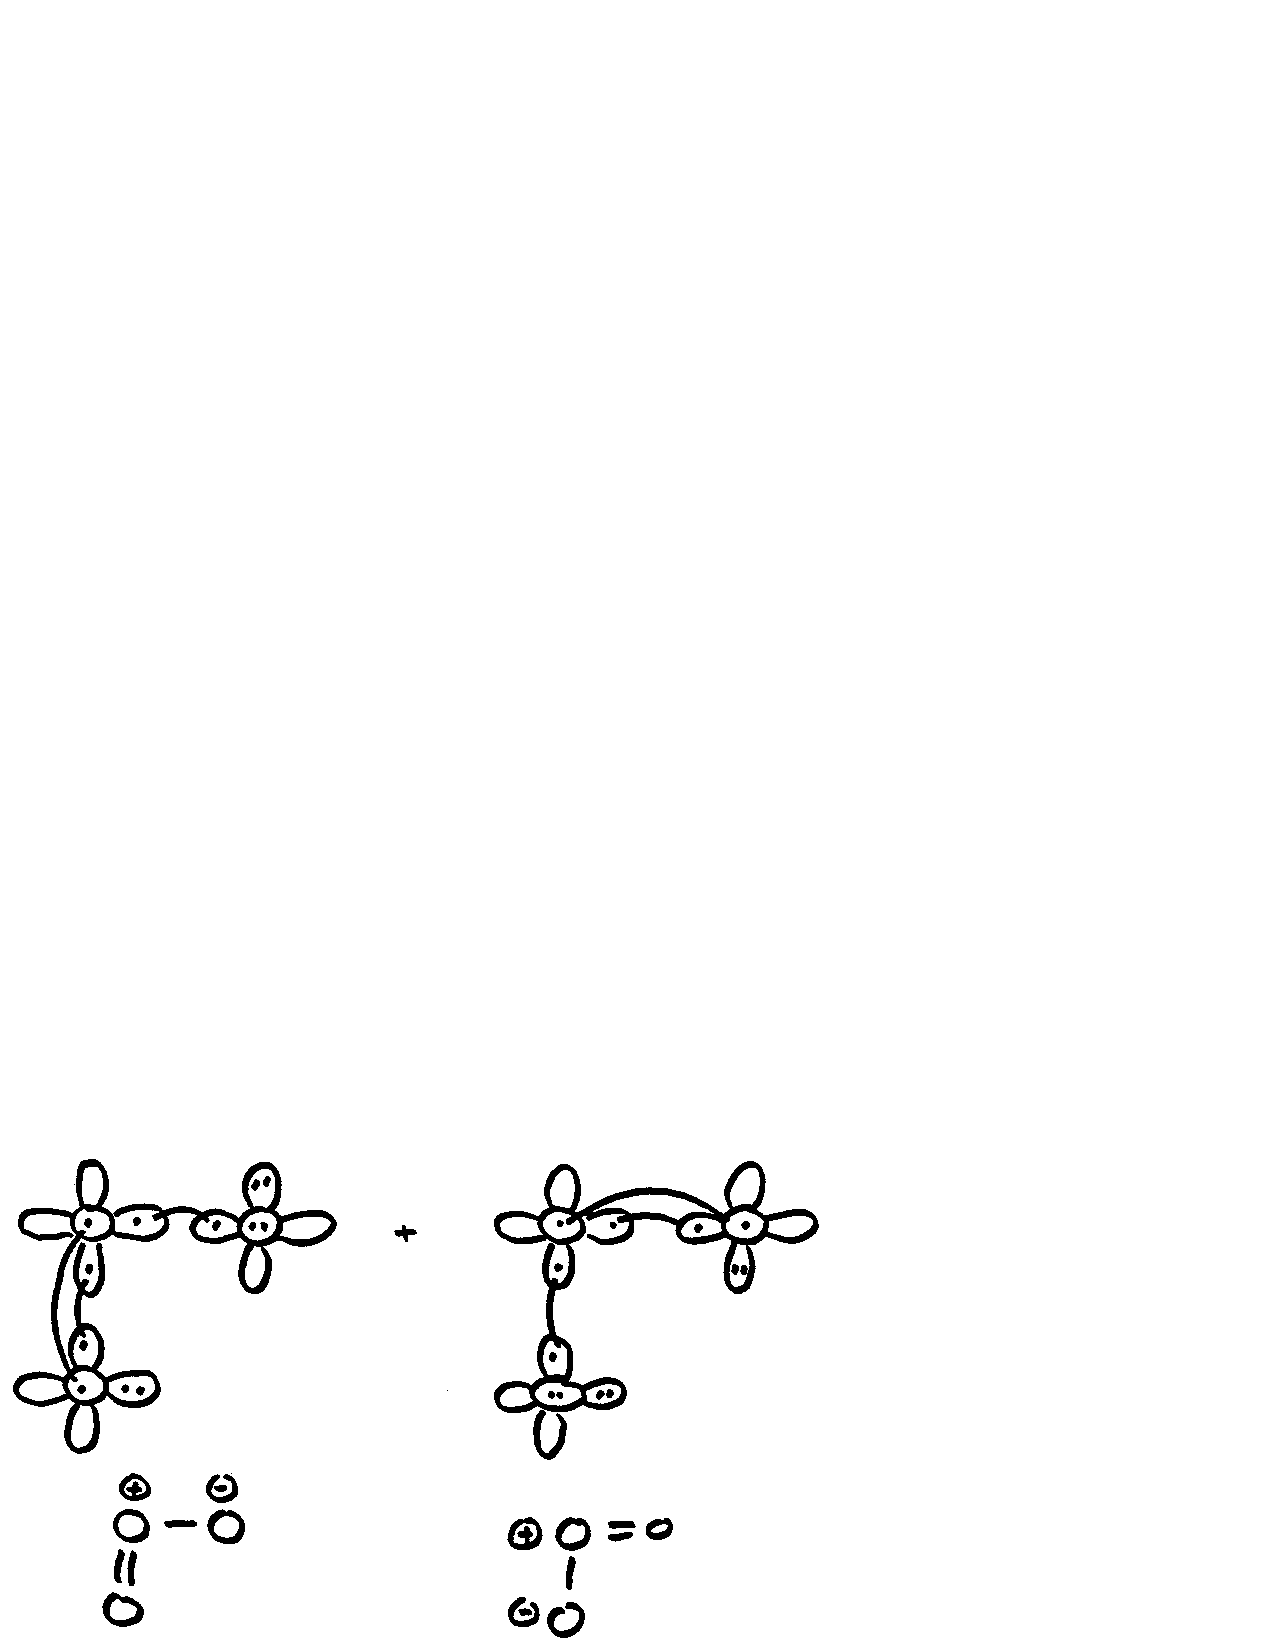
\includegraphics{fg11-u}
\end{equation}
This is a somewhat extreme, but essentially correct, view of the bonding.

\section{Diazomethane}

Consider bonding H$_2$C and two N atoms.  One form, diazirine, is
\begin{equation}
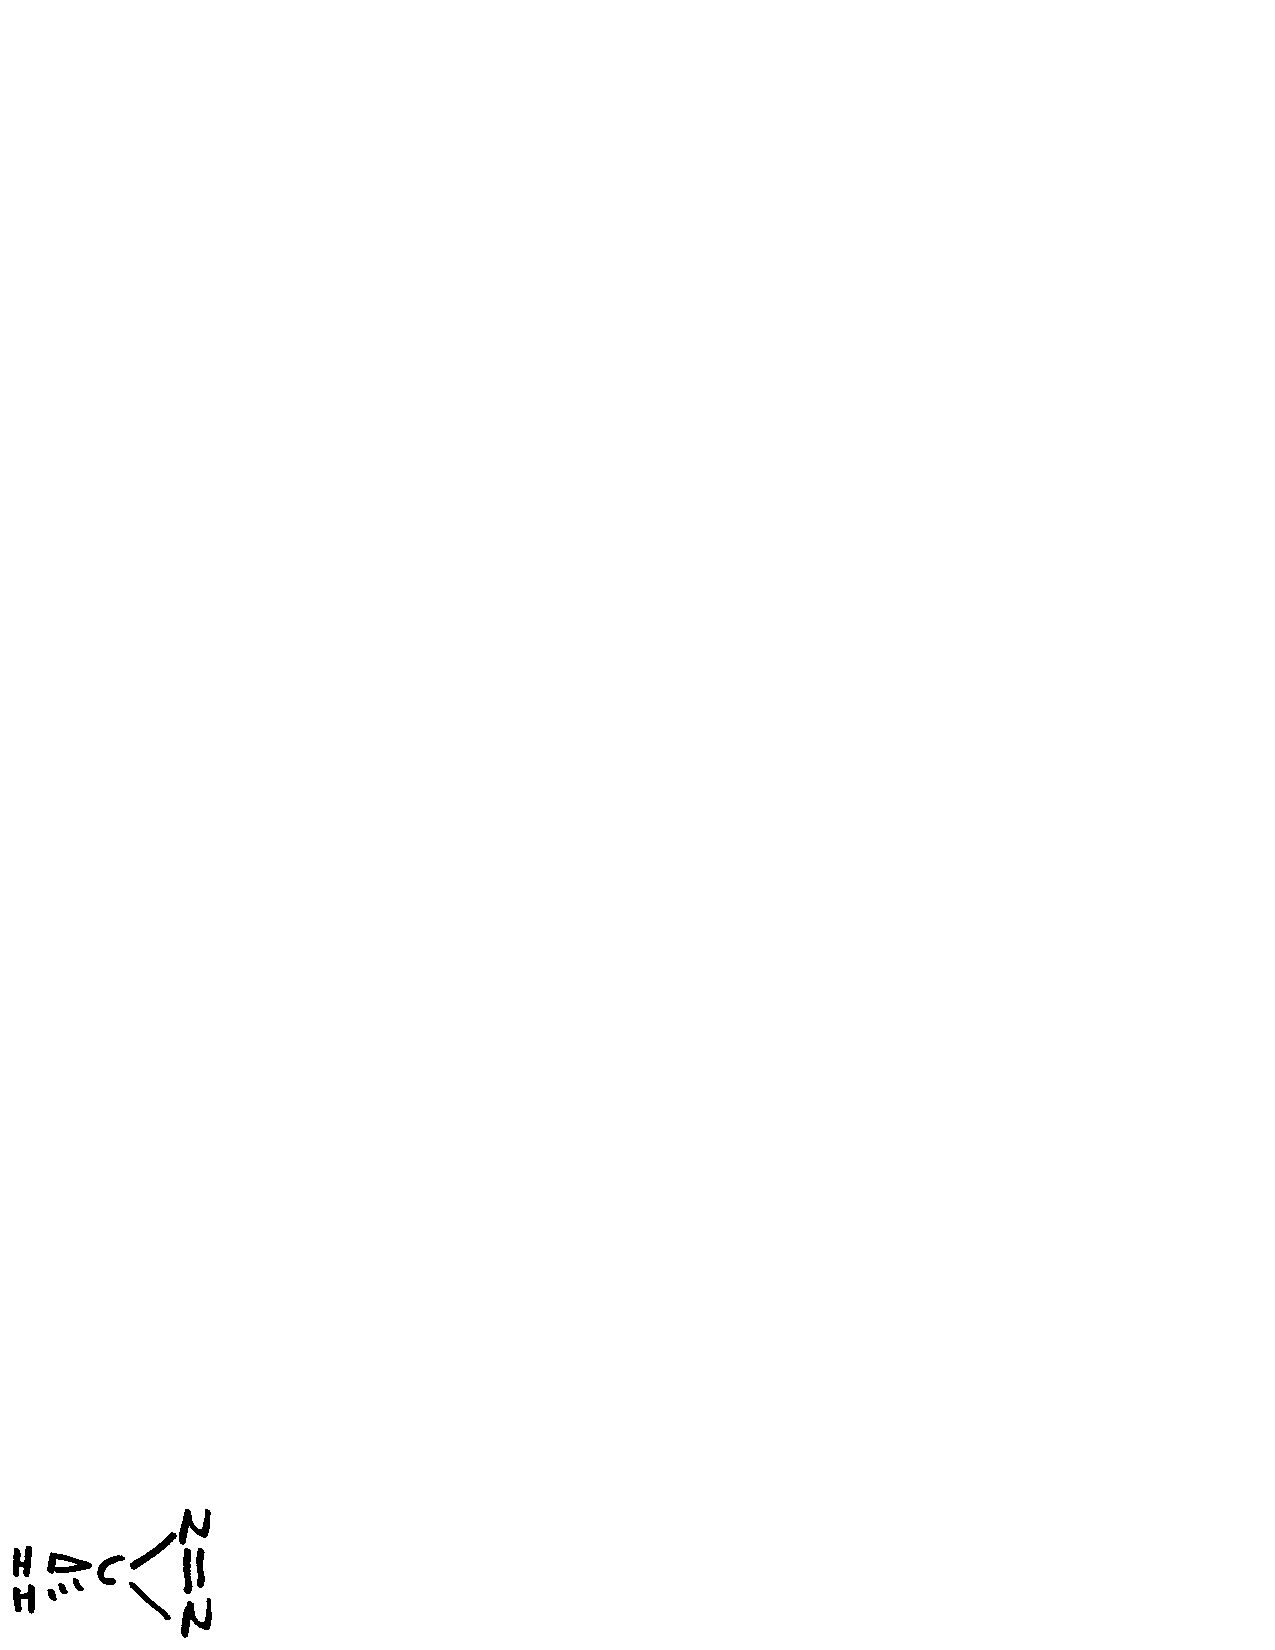
\includegraphics{fg11-v}
\end{equation}
However, the bad bond angles tend to destablize this form.  A second 
form, called diazomethane, can be envisioned in terms of the three pieces
\begin{equation}
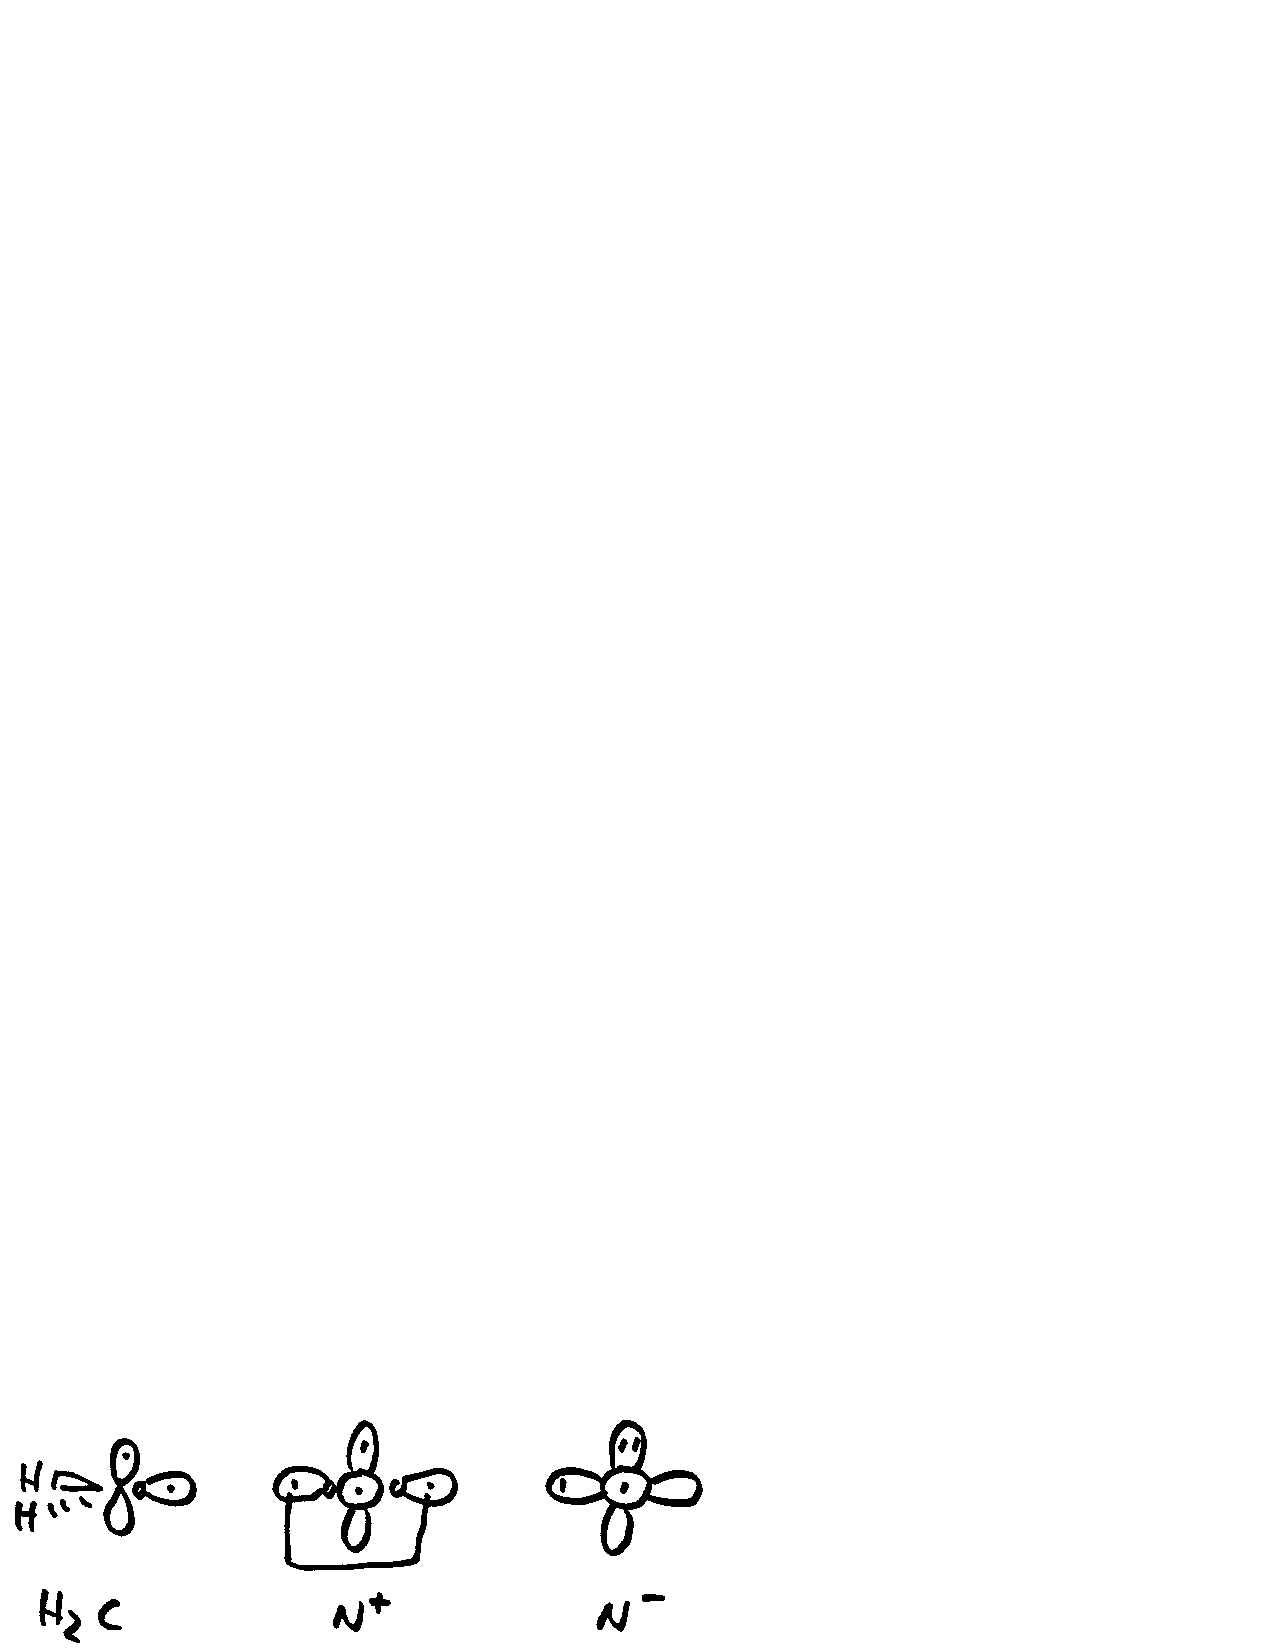
\includegraphics{fg11-w}
\end{equation}
leading to
\begin{equation}
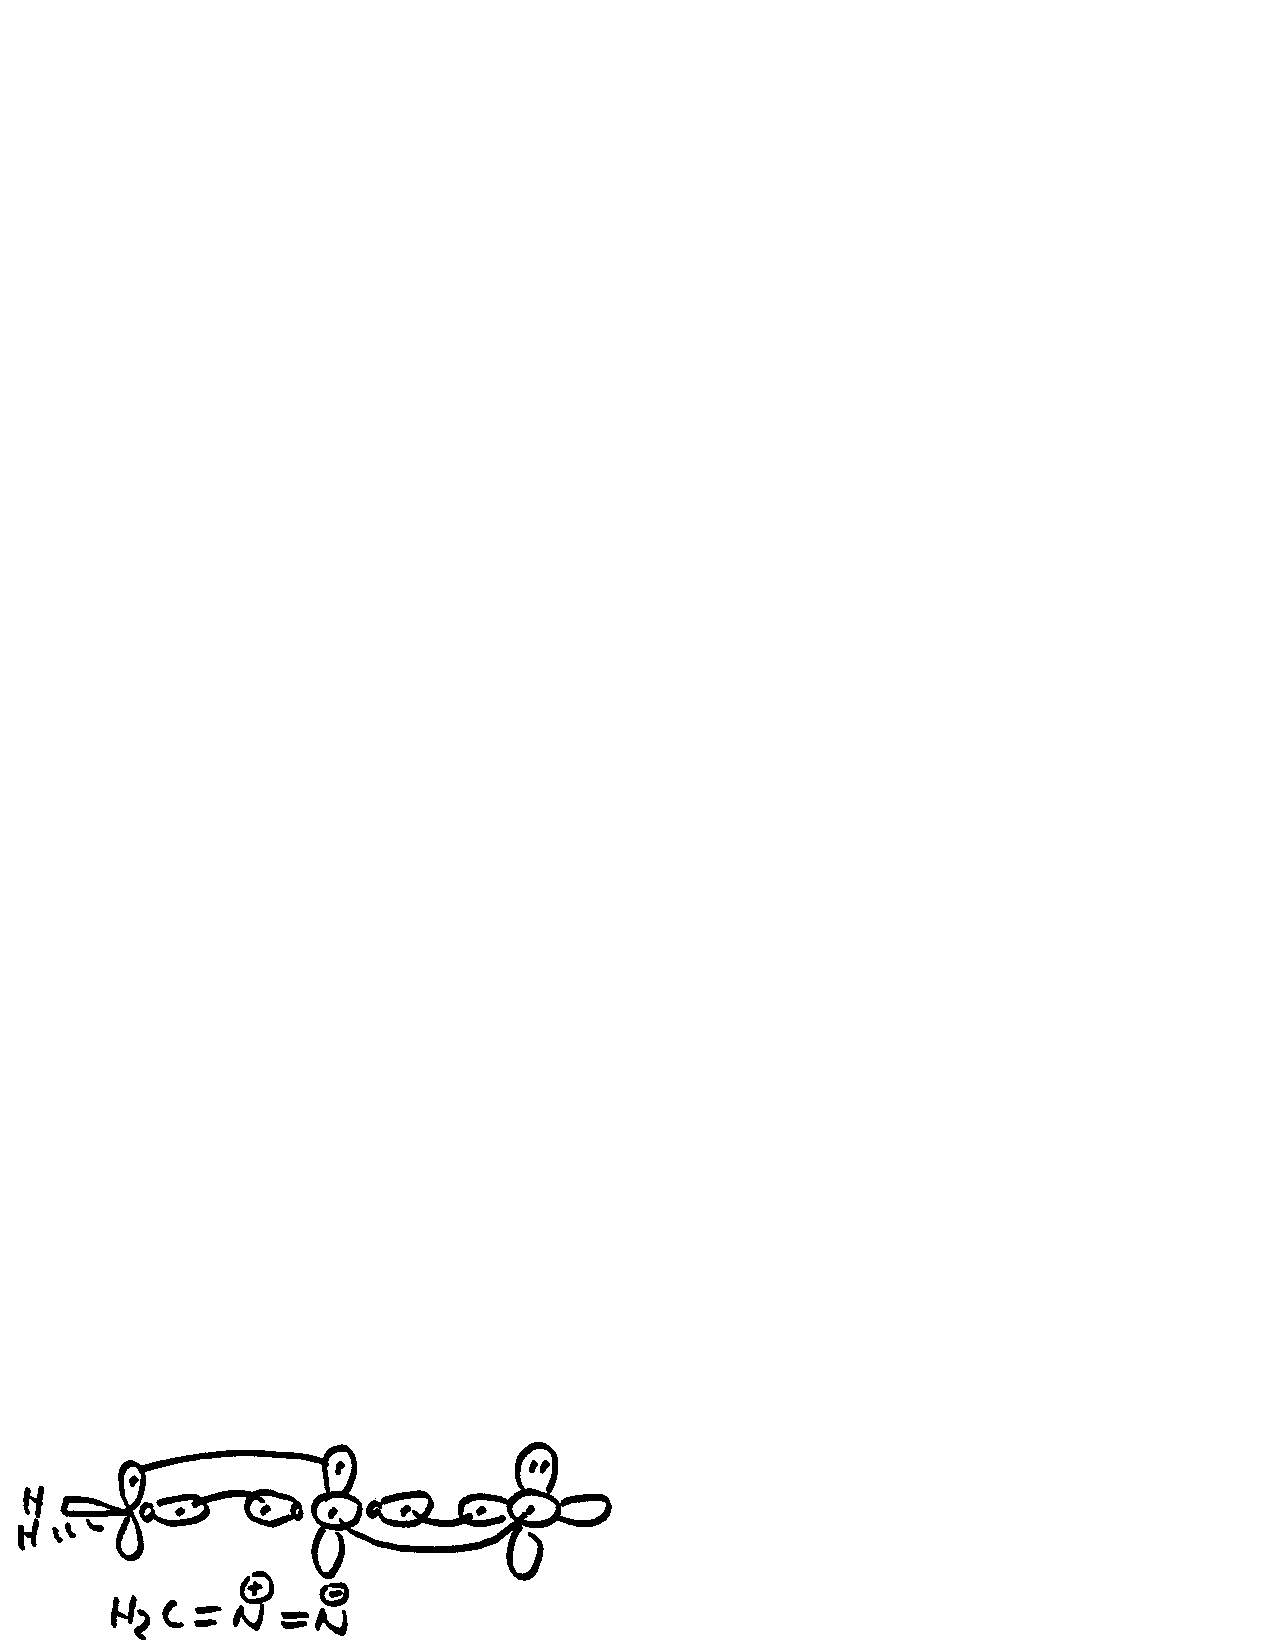
\includegraphics{fg11-x}
\end{equation}
Thus, by ionizing the central N we obtain four orbitals that can form 
covalent bonds leading to two double bonds.  The outer N has available 
a singly-occupied orbital for this electron allowing stabilization of 
the charge.

%%%% RPM Note
% What is included but unlabeled in my set of the notes (Molecular
% Crystals) was once labeled chapter 9. Carol had 
% inserted these sections at the end of the current chapter 9
% (ionic bonding), but it really doesn't belong there. I am putting
% it at the end of this section. Since both talk about hypervalency
% and wierd bonding.

\section{Molecular Crystals}

For closed shell atoms or molecules there are only weak interactions
responsible for condensation.  Consequently, boiling temperatures are
generally low and packing tends to be closest packed.  The following
sections are examples to be considered.

\subsection{Noble Gases}

The crystals of Ne, Ar, Kr, and Xe are all face-centered cubic with 
geometries as listed in Table \ref{chap9-tab23}.  For Ar a metastable hexagonal 
close-packed phase has been formed at $T = 2$ to 80$^{\circ}$K, but it 
transforms to face-centered cubic upon cold working.

At atmospheric pressure, He does not crystallize.  The melting point is 
4.215$^{\circ}$K, and below 2.172$^{\circ}$K, He becomes a superfluid.  
All discussions are based on $^4$He, which is more than 99.999 percent 
of natural He.  The other isotope, $^3$He has somewhat different 
properties.  At increased pressures, three crystalline 
forms of He have been prepared:
\begin{enumerate}
\item $\alpha$, hexagonal close-packed.  For $T = 1.2^{\circ}$K,  
hexagonal close-packed is stable at $p > 25$ atm.  For $T = 4.2^{\circ}$K,
hexagonal close-packed is stable at $p > 300$ atm.  For $T = 15^{\circ}$K, 
hexagonal close-packed is stable at $p > 1000$ atm.  At 1.4$^{\circ}$K and 
$p = 26$ atm, the bond distance is 3.663 \AA, which distance is 2.58 
percent larger than in body-centered cubic for the same $T$ and $p$.

\item $\beta$, face-centered cubic.  Above $T = 15^{\circ}$K, the 
crystalline form of He is face-centered cubic, which is stable
for $p > 1200$ atm at 15$^{\circ}$K and $p > 1800$ atm at 20$^{\circ}$K.

\item $\gamma$, body-centered cubic.  The form is stable in a 
narrow region of $T$ and $p$ between 1.5 and 1.8$^{\circ}$K.  In this range of
temperatures, body-centered cubic is the lowest pressure crystalline 
form. The pressure range of stability is 1/2 atm,
above which hexagonal close-packed is stable.  At 1.4$^{\circ}$K and 
$p =$ 20 atm, the bond distance is 3.571 \AA.
\end{enumerate}

Some properties of solid inert gases are listed in Table
\ref{chap9-tab14}. The bond distance can be compared directly with
that in the dimer, as in Table \ref{chap9-tab15}.  For Ne and Ar the
bond distances in the dimer and crystal are the same, within
experimental error.  However, for Kr and Xe, the crystal values are
about 0.03 \AA\ shorter.  On the other hand, even at 26 atm of
pressure, crystalline He leads to a bond length 0.6 \AA\ longer than
He$_2$.  At its boiling point, liquid He has an average bond distance
1.19 \AA\ longer than the dimer.  Based on a liquid density of 125
kg/cm$^3$ and assuming each atom of the liquid has twelve neighbors.

\begin{table}
\caption{Crystalline properties of noble gases.$^a$}
\label{chap9-tab14}
\begin{tabular}{ccccccccc}\\ \hline

&Crystal&Bond&\multicolumn{3}{c}{Triple Point}
&Boiling&$\Delta$H$_{vap}$\cr
&Structure$^b$&Distance&&&&Point&(cal)\cr
& & 0$^{\circ}$K & T$_t$ & p & $\Delta$H$_m$ & 
T$_{bp}$&0$^{\circ}$K&$T_{bp}$\cr
& & (\AA)$^b$&($^{\circ}$K)&(atm)&(kcal)&($^{\circ}$K)&(ideal)\cr

He & (hcp)$^d$ & 3.663$^d$ & - & - & - & 4.215 & 0.0143 & 0.020\cr
Ne & (fcc) & 3.155 & 24.553 & 0.4277 & 0.0793 & 27.096 & 0.447 & 
0.414\cr
Ar & (fcc) & 3.755 & 83.81 & 0.6801	& 0.284 & 87.30 & 1.848 & 1.541\cr
Kr & (fcc) & 3.991 & 115.78 & 0.7220 & 0.392 & 119.80 & (2.648) & 
2.158\cr
Xr & (fcc) & 4.336 & 161.36 & 0.8059 & 0.549 & 165.03 & 3.798 & 
3.020\cr
Rn & & 202$^c$ &&(0.69)&211&4.995&(3.921)\cr
\hline
\end{tabular}\\
$^a$ Based on reference 2, unless indicated otherwise.
$^b$ Reference 4.
$^c$ Melting point. 
$^d$ At 1.4$^{\circ}$K, and $p = 20$ atm.
\end{table}

\begin{table}
\caption{Bond distances, in \AA.}
\label{chap9-tab15}
\begin{tabular}{ccc}\\ \hline
& Dimer & Crystal\cr

He & 3.03 & 3.663\cr
Ne & 3.1$^{\underline{5}}$ & 3.155\cr
Ar & 3.758 & 3.755\cr
Kr & 4.03 & 3.991\cr
Xe & 4.34$^{\underline{1}}$ & 4.336\cr
\hline
\end{tabular}
\end{table}

\begin{table}
\caption{Energetic quantities, in kcal.}
\label{chap9-tab16}
\begin{tabular}{ccccc}\\ \hline
& Dimer Bond &\multicolumn{2}{c}{Crystal}&$\Delta H_{vap}$\cr
& Energy & $\Delta H_{fusion}$ & $\Delta H_{vap}$ & $\Delta 
H_{dimer}$\cr

He & 0.02 & -- & 0.0143 & 0.7\cr
Ne & 0.047 & 0.08 & 0.45 & 9.6\cr
Ar & 0.24 & 0.28 & 1.85 & 7.7\cr
Kr & 0.36 & 0.39 & 2.65 & 7.4\cr
Xe & 0.53 & 0.55 & 3.80 & 7.2\cr
Rn & & 0.69 & 5.00\cr
\hline
\end{tabular}
\end{table}

The cohesive energy of the crystal should be related to the bond
energy in the dimer.  Indeed, as indicated in Table \ref{chap9-tab16}
for Ar, Kr, and Xe, the cohesive energy, at 0$^{\circ}$K, is $7.4 \pm
0.2$ times the dimer energy.  Since each atom of the crystal has
twelve near neighbors, we would expect the cohesive energy to be
around six times the dimer energy, correcting for double counting.
This suggests the possible importance of three-body terms in the
crystal.  For Ne, the cohesive energy of the crystal is 9.6 times that
of the dimer.  Perhaps the current bond energy of Ne$_2$ is too small,
an increase of D$_0$ to 0.061 kcal instead of 0.047 would change the
ratio to 7.4.

On the other hand, the cohesive energy of liquid He is less than that of He 
dimer, suggesting nonadditive forces in the liquid.  Perhaps the difference 
between He and the other inert gases is related to the difference in the 
valence shell, $(1s)^2$ for He and $(np)^6$ for the others.  Or, perhaps the
weak bonding in He and light mass, leading to large zero-point energy 
effects, is involved.

\subsection{The Heavy Halogens}

\subsubsection{Crystalline Compounds}

\begin{figure}
% missing figure
%\includegraphics[scale=0.75]{fg9-}
\caption{}
\label{chap9-fig}
\end{figure}

The molecules Cl$_2$, Br$_2$, and I$_2$ crystallize with the
structure, type A14, indicated in Figure \ref{chap9-fig14}.
Characteristic distances are listed in Table \ref{chap9-tab17}.  Here
we see that the intermolecular bond distances change less than 0.01
\AA\ from the value for the free molecule.

\begin{table}
\caption{Bond distances, in \AA, for crystalline halogens.}
\label{chap9-tab17}
\begin{tabular}{ccccccccc}\\ \hline
&Diatomic&Temperature&\multicolumn{6}{c}{Crystalline Halogens}\cr
& & ($^{\circ}$K) & 1-2 & 2-3 & 2-4 & 2-5 & 2-6 & 2-7\cr

Cl$_2$ & 1.988 & 113 & 1.98 $\pm$ 0.02 & 3.32 & 3.82 & 3.74 & 3.84 & 
3.97\cr
Br$_2$ & 2.281 & 123 & 2.27 $\pm$ 0.10 & 3.32 & 3.80 & 3.99 & 4.02 & 
4.14\cr
I$_2$ & 2.666 & 110 & 2.715 $\pm$ 0.006 & 3.50 & 3.97 & 4.34 & 4.27 & 
4.41\cr
& & 298 & 2.69 & 3.56 & 4.06 & 4.40 & 4.36 & 4.48\cr
\hline
\end{tabular}
\end{table}

A particularly short bond distance occurs for the configuration
\begin{equation}
% missing figure
%\includegraphics{fg9-}
\label{chap9-eqno16}
\end{equation}
Recalling the orbital configuration for Cl$_2$
\begin{equation}
% missing figure
%\includegraphics{fg9-}
\label{chap9-eqno17}
\end{equation}
we see that this short distance corresponds to the interaction of a 
singly-occupied bond orbital, $\sigma$, of one Cl with a doubly-occupied 
nonbonding orbital, $\pi$, on the adjacent Cl, the $\sigma - \pi$ 
interaction.  Whereas the other intermolecular bond distances involve 
interaction of two doubly-occupied $\pi$ orbitals, the $\pi-\pi$ 
interaction.  Thus, it is reasonable that the $\sigma-\pi$ should lead to more
favorable interaction and shorter bonds than $\pi-\pi$.  One might 
think of the $\sigma-\pi$ interaction as involving some delocalization of 
the $\pi$ orbital on one Cl$_2$ into the $\sigma$ system of the adjacent 
Cl$_2$. This is equivalent to allowing some charge transfer character of 
the form
\begin{equation}
% missing figure
%\includegraphics{fg9-}
\label{chap9-eqno18}
\end{equation}
a situation not possible for the $\pi-\pi$ case, since both orbitals 
are already doubly-occupied.

For crystalline I$_2$, the intra-atomic bond distance at low temperature, 
110$^{\circ}$K, 2.715 $\pm$ 0.006 \AA, is significantly longer than for 
free I$_2$, 2.666 \AA.  This increase is consistent with some degree
of charge transfer arising from the $\sigma-\pi$ intermolecular 
interaction.  For high temperature, 298$^{\circ}$K, molecular vibrations 
lead to an increase in the intermolecular distances, and hence, a decrease in
the $\sigma-\pi$ interaction, resulting in a decrease in the I-I distance 
toward the free molecule value, see Table \ref{chap9-tab17}.

Considering the assembly of Cl$_2$ molecules in the plane, we see that 
all $\pi$ orbitals get stabilized.  This should lead to a net 
contraction, and hence,
\begin{equation}
% missing figure
%\includegraphics{fg9-}
\label{chap9-eqno19}
\end{equation}
to shorter than usual $\pi-\pi$ interactions.  This seems to be the 
case.  Thus, Br$_2$ and I$_2$ lead to larger distances for $\pi-\pi$ 
interactions of molecules in different planes than for molecules in 
the same plane.  From these considerations, we expect that the easy 
cleavage planes should be between layers, as observed.

Recent experiments$^{10}$ on dimers of Cl$_2$, i.e., (Cl$_2$)$_2$,
show that the dimer has a dipole moment, a result consistent with the
configuration (\ref{chap9-eqno16}) and indicating a favorable
$\sigma-\pi$ interaction.

In Table \ref{chap9-tab18} we see that the energy of vaporization from
halogen crystals, per X$_2$ molecule, increases from 7.2 to 10.9 to
15.6 kcal for Cl$_2$ to Br$_2$ to I$_2$.  This suggests increased
$\sigma-\pi$ interactions from Cl to Br to I, as seems consistent with
the structures, see Table \ref{chap9-tab17}.

\begin{table}
\caption{Properties of X$_2$ crystals.}
\label{chap9-tab18}
\begin{tabular}{cccccc}\\ \hline

& $\Delta H^a_{vap}$ &\multicolumn{3}{c}{Triple Point}\cr
& 0$^{\circ}$K & T$_t$ & p & $\delta H_m$$^a$ & $T_{bp}$\cr
& (kcal) & ($^{\circ}$K) & (atm.) & (kcal) & ($^{\circ}$K)\cr

F$_2$$^b$ & 1.008 & 53.48 & 0.00249 & 0.0610 & 84.95\cr
Cl$_2$ & 3.608 & 172.16 & 0.01348 & 0.7655 & 239.10\cr
Br$_2$ & 5.465 & 265.90 & 0.0587 & 1.2635 & 332.25\cr
I$_2$ & 7.828 & 386.7 & 0.1195 & 1.870 & 458.4\cr
\hline
\end{tabular}\\
$^a$ $\Delta H$ is per atom of F. 
$^b$ $T_{\alpha \beta} =$ 45.55$^{\circ}$K, $\Delta H_{\alpha 
\beta} =$ 0. 0870 kcal.
\end{table}

\subsubsection{Hypervalent Compounds}

Compounds such as
\begin{equation}
% missing figure
%\includegraphics{fg9-}
\end{equation}
and
\begin{equation}
% missing figure
%\includegraphics{fg9-}
\end{equation}
are quite stable. This involves bonding configurations of the form
(\ref{chap9-eqno20a})
\begin{equation}
% missing figure
%\includegraphics{fg9-}
\label{chap9-eqno20a}
\end{equation}
which are stabilized by charge transfer configurations of the form
(\ref{chap9-eqno20b}) and will be discussed later.
\begin{equation}
% missing figure
%\includegraphics{fg9-}
\label{chap9-eqno20b}
\end{equation}

\subsection{O$_2$ and F$_2$}

This section discusses the three stable crystalline forms of O$_2$ and 
the two crystalline forms of F$_2$, at 1 atm.

\subsubsection{$\alpha$O$_2$}

$\alpha$O$_2$ is end-centered, monoclinic, has two O$_2$ per cell, and
is stable below 23.86$^{\circ}$K.  It consists of closed-packed layers
of O$_2$ with the O$_2$ axis perpendicular to the plane.  The
experimental orientation is 4-1/2$^{\circ}$ tilt in the $x$ direction,
with an uncertainty of 8$^{\circ}$.  These layers are stacked abcabc,
like face-centered cubic, as in Figure \ref{chap9-fig16}(a).  There is
a slight distortion of the close-packed plane, as indicated in Figure
\ref{chap9-fig16}(b), leading to a unit cell with two molecules.
Neutron diffraction studies indicate that the spin of the corner atoms
is antiferromagnetically coupled to the spin of the central atoms, to
obtain a net spin of zero.


\begin{figure}
% missing figure
%\includegraphics[scale=0.75]{fg9-16}
\caption{}
\label{chap9-fig16}
\end{figure}

The X-ray diffraction studies lead to a bond distance of 1.15 $\pm$ 
0.12 \AA\ for the intramolecular bond, which is within experimental 
error of the free molecule value, 1.208 \AA.  Assuming an 0-0 bond of
1.208 \AA\ perpendicular to the $xy$ plane leads to the following distances, 
starting with the upper atom at the center of a cell:
\begin{enumerate}
\item two at 3.15 \AA, lower atoms of corner molecules in unit cell 
of $b$ layer

\item one at 3.21 \AA, lower atom of center molecules in unit cell of 
$b$ layer

\item four at 3.20 \AA, upper atoms of corner molecules in unit cell 
of $a$ layer

\item two at 3.43 \AA, upper atoms of center molecules of adjacent 
molecules of $a$ layer

\item four at 3.42 \AA, lower atoms of corner molecules in unit cell 
of $a$ layer.
\end{enumerate}

\subsubsection{$\beta$O$_2$}

$\beta$O$_2$ is rhombohedral, hexagona, has one O$_2$ per cell, and is 
stble between 23.86 and 43.79$^{\circ}$K.  This is similar to 
$\alpha$O$_2$ except that the closest packed layer is undistorted, no 
antiferromagnetic coupling.  The results is six equivalent neighbors 
in the same plane at 3.31 \AA, compared with four at 3.20 \AA, and two 
at 3.43 \AA\ for $\alpha$O$_2$, an average of 3.38 \AA, and three 
neighbors in the next plane at 3.18 \AA, compared with two at 3.15 
\AA, and one at 3.21 \AA\ for $\alpha$O$_2$, an average of 3.17 \AA.

\subsubsection{$\gamma$O$_2$}

$\gamma$O$_2$ is cubic, has eight O$_2$ per cell, and is stable from 
43.79$^{\circ}$K to the melting point, 54.35$^{\circ}$K.  The 
structure of $\gamma$O$_2$ is illustrated in Figure \ref{chap9-fig17}.

\begin{figure}
% missing figure
%\includegraphics[scale=0.75]{fg9-}
\caption{}
\label{chap9-fig17}
\end{figure}

This is called the A15 crystal structure and is the one associated
with high temperature superconductors.  The circles indicate randomly
oriented O$_2$ molecules in three dimensions. The arrows indicate
O$_2$ that are randomly oriented in two dimensions; each arrow
represents a degree of freedom in the plane shown. Thus, ????
indicates motion in the plane of the paper, whereas $\leftrightarrow$
and $\updownarrow$ indicate motion in a plane perpendicular to the
paper.

At the corners and center of a cube are type I O$_2$ molecules that
are randomly oriented in three dimensions.  On each face of the cubic
unit cell are two type II O$_2$ molecules with random orientations in
two dimensions, the molecules of a pair on one face must be
perpendicular to the line connecting the pair.  All together, one
cubic cell consists of two type I molecules and six type II molecules.
Around each type I molecule are twelve type II at a distance of 3.82
\AA, center-to-center.  Around each type II molecule are: two type II
at 3.42 \AA, 1-2 in Figure \ref{chap9-fig3}; four type I at 3.82 \AA,
1-3 and 1-6 in Figure \ref{chap9-fig3}; and, eight type II at 4.18
\AA, 1-4 and 1-5 in Figure \ref{chap9-fig3}.

Actually these motions are not entirely random. There must be coupling
of the motions in order to avoid very short intermolecular O-O
distances.  For example,
\begin{enumerate}
\item if molecules 1 and 5, in Figure \ref{chap9-fig17}, are both oriented in 
the $z$ direction, perpendicular to the plane, the closest O-O
distance is 3.28 \AA;

\item if molecules I and 3, in Figure \ref{chap9-fig17}, are both oriented in 
the $x$ direction, the shortest O-O distance is 2.79 \AA, and

\item if molecule 3 is in the $y$ direction while 1 is in the 
$x$ direction, the shortest O-O distance is 3.03 \AA. Consequently, if 
1 is in the $x$ direction, 3 will tend to be in the $z$ direction.
\end{enumerate}

The thermodynamic properties of condensed O$_2$ are given in Table 
\ref{chap9-tab19}.  

\begin{table}
\caption{Thermodynamic properties of condensed O$_2$.}
\label{chap9-tab19}
\begin{tabular}{cccc}\\ \hline

& T & $\Delta H^a$ & p\cr
& ($^{\circ}$K) & (kcal) & (atm)\cr

$\alpha \beta$ Transition & 23.86 & 0.01156 & --\cr
$\beta \gamma$ Transition & 43.79 & 0.08875\cr
Triple Point & 54.35 & 0.0532 & 0.00148\cr
Boiling Point &	90.18 & 0.815\cr
$\Delta H_{v,O^{\circ}K}$ & & 1.048\cr
\hline
\end{tabular}\\
$^a$ per atom of O.
\end{table}

\subsubsection{$\alpha$F$_2$}

$\alpha$F$_2$ is monoclinic, stable below 45.6$^{\circ}$K, and is 
similar to $\alpha$O$_2$.  It consists of nearly close-packed layers 
of F$_2$ molecules with the axis tipped 18 degrees from the normal.  
These layers are stacked abc as in an face-centered cubic array, but 
with alternate layers tilted in the opposite directions, as shown in 
Figure \ref{chap9-fig18}.

\begin{figure}
% missing figure
%\includegraphics[scale=0.75]{fg9-}
\caption{}
\label{chap9-fig18}
\end{figure}

This structure is the same as for $\alpha$O$_2$ except $\alpha$F$_2$ 
has the molecule tilted in the $y$ direction.  The close-pkaced layers 
are stacked abcabc, but with tilts $\downarrow \uparrow \downarrow 
\uparrow \downarrow \uparrow$.

The intermolecular bond length is found to be 1.49 \AA, which is probably 
within experimental error of the value for the free molecule, 1.41 
\AA.  The distances are indicated in Figure \ref{chap9-fig19}.  There are three
short intermolecular distances, 2.82 to 2.87 \AA, and nine longer
ones, 3.17 to 3.78 \AA.  Note that the projection of the 18 degrees
tilt upon the $y$ axis is 17.6 degrees, and the projection on the $x$
axis is $-$4 degrees, using an orthogonal coordinate system rather
than the usual monoclinic coordinate system.

\begin{figure}
% missing figure
%\includegraphics[scale=0.75]{fg9-}
\caption{}
\label{chap9-fig19}
\end{figure}


\subsubsection{$\beta$F$_2$}

For $\beta$F$_2$, cubic, is stable from 45.6$^{\circ}$K to the melting
point, 53.5$^{\circ}$K, and is the same as $\gamma$O$_2$.
$\beta$F$_2$ has the same crystal structure as $\gamma$O$_2$, see
Figure \ref{chap9-fig17}.  There are eight molecules per cubic unit
cell. at the corners and center of a cubi unit cell are type I F$_2$
molecules, randomly oriented in three dimensions.  On each face, of
the cubic unit cell, are two type II F$_2$ molecules with random
orientation in two dimensions.  The distances from center-to-center
are:

\begin{enumerate}
\item \emph{Type I} twelve type II neighbors at 3.73 \AA
\item \emph{Type II} two type II neighbors at 3.34 \AA
\item four type I neighbors at 3.73 \AA
\item eight type II neighbors at 4.08 \AA
\end{enumerate}

Just as in $\gamma$O$_2$, the rotations of the F$_2$ must be 
hindered, since very short F-F intermolecular bond distances arise 
from some orientations.

\subsubsection{Comparison with O$_2$}

Comparing the crystal structure of F$_2$ and O$_2$, we see that the 
intermolecular distances in O$_2$ are 0.08 to 0.10 \AA\ larger than in 
F$_2$, indicating a slightly larger size for O atom as compared with F 
atom.  Of course, the 
bond length of O$_2$, 1.208 \AA, is
shorter than that of F$_2$, 1.412 \AA\ because of the pi bonding.

\subsection{Crystal Structures of N$_2$}

There are two crystalline forms of N$_2$ stable at atmospheric 
pressure.  First, $\alpha$N$_2$ has a cubic crystal
structure with four N$_2$ per cell and is stable below 35.6 K.  
Second, $\beta$N$_2$ has a hexagonal crystal structure
with two N$_2$ per cell and is stable from 35.6 K to the melting point. 

Another form, $\lambda$N$_2$, with a
tetragonal unit cell, and two N$_2$ per cell, is stable at high 
pressure, above 4 kbar.

For thermodynamic properties of condensed N$_2$, see Table \ref{chap9-tab22}.

\begin{table}
\caption{Thermodynamic properties of condensed N$_2$.}
\label{chap9-tab22}
\begin{tabular}{cccc}\\ \hline

& T & $\Delta H$ & p\cr
& (K) & (kcal) & (atm)\cr

$\alpha \beta$ Transition & 35.61 & 0.0278 & --\cr
Triple Point & 63.14 & 0.08615 & 0.1235\cr
Boiling Point & 77.35 & 0.6675\cr
$\Delta H_{v,0^{\circ}K}$ & 0.8305\cr
\hline
\end{tabular}
\end{table}

\subsubsection{$\alpha$N$_2$}

The N$_2$ molecules are arranged in an face-centered cubic structure with 
the four N$_2$ of a cubic unit cell each oriented
along a different three-fold axis.  There is currently a disagreement 
concerning the crystal structure
with two possible cases:

\begin{enumerate}
\item  Undistorted, Pa 3 space group.  The molecular 
centers are at the lattice points for face-centered cubic . This leads to 
interatomic distances of six atoms at 3.582 \AA\ and six atoms at 
3.637 \AA.

\item Distorted, P2$_1$ 3 space group.  The molecular centers
are moved 0.17 \AA\ along the three-fold axes.  This leads to two types of 
molecules in the unit cell, two of each, with interatomic distances as
\begin{enumerate}
\item \emph{Type I} three II at 3.428 \AA
\item six I at 3.556 \AA
\item three II at 3.737 \AA
\item \emph{Type II} three I at 3.428 \AA
\item six II at 3.724 \AA
\item three I at 3.737 \AA
\end{enumerate}

\end{enumerate}

\subsubsection{$\beta$N$_2$}

The N$_2$ molecules are arranged in a hexagonal close-packed structure with 
the molecular axis oriented at 56.0 $\pm$ 2.5 degrees from the
six-fold axis, the $\bot$ to the closed-packed planes.  There are two possible 
cases, which cannot yet be
distinguished.  One is that each N$_2$ axis precesses about the six-fold 
axis, and the other is that there is a statistical distribution among
six orientations about the axis.  The center-to-center distances are 
six at 4.046 \AA\ and six at 4.055 \AA.

\subsection{Condensed H$_2$}

\subsubsection{Crystal Structures of H$_2$}

The high temperature form of crystalline H$_2$ is an hexagonal 
close-packed structure with nearly free rotation, like $\beta$N$_2$.
Below about 1.5$^{\circ}$K, depending upon ortho-para ratio, there 
is a transition to a cubic structure.  Often this is suggested to be an 
face-centered cubic  arrangement of freely rotating H$_2$.  However,
some studies suggest that this cubic form may be like $\alpha$N$_2$ with 
orientational preferences.  The molecular
diameters, in \AA, are as follows, for T = 3 to 4$^{\circ}$K,$^6$:
\begin{tabular}{cccc}
& H$_2$ & HD & D$_2$\cr
Cubic & 3.77 & 3.66 & 3.59\AA\cr
HCP & 3.77 & 3.64 & 3.60\AA\cr
\end{tabular}
Since the bond length of H$_2$ is 0.74 \AA\ these values suggest a van der Waals 
radius of about 1.51 \AA\ about each H atom.

\subsubsection{Ortho-Para H$_2$}

Hydrogen exhibits a peculiar dependence upon nuclear spin state that is 
worthy of note.  The electronic state of H$_2$ is ${^1\Sigma}^+_g$, which 
is invariant under all symmetry operations.  Considering
nuclear motion, the total wavefunction can be written as
$$
\Psi^{e \ell} (r) \Psi^{vibn}_v (R) \Psi^{rotn}_{JM}( \theta , 
\varphi ),
$$
where the vibrational wavefunction depends only on internuclear 
distance, $R$, and the rotational wavefunction depends only on 
orientation, $\theta , \varphi$.  Thus, $\Psi^{vibn}$ is invariant 
under inversion.  On the other hand, inversion changes $\theta$ to 
$\pi - \theta$, and $\varphi$ to $\varphi + \pi$, with the result that
$\Psi^{rotn}_{JM}$ changes to $(-1)^J \Psi^{rotn}_{JM}$.  
Thus, even $J$ are gerade and odd $J$ are ungerade.

The dependence of energy upon $J$ is given by $E_J = B_0 J(J + 1)$,
where $B_0 =$ 59.322 cm$^{-1}$.  Thus, ignoring nuclear spin effects, below 
20.268$^{\circ}$K, the boiling point of H$_2$, 99.9 percent of the H$_2$ 
should be in the lowest rotational level, $J = 0$.

The nucleus of H atom has spin equal to one-half, and hence, the nuclear 
spins can be coupled into a net nuclear
spin of $I = 0$, or $I + 1$.  Just as with electrons, the $I = 0$ state is 
antisymmetric, called para, under
interchange of nuclear spins, while the $I = 1$ state is symmetric, called 
ortho.  However, protons are
fermions and hence, interchange of the protons, spatial and spin 
coordinates, must change the sign
of the wavefunction.  Since inversion interchanges the nuclei, we see that
$J$ equals even, must go with $I = 0$, para, and $J$ equals odd, must 
go with $I = 1$, ortho.

At high temperature 3/4 of the H$_2$ molecules would be ortho, based
on nuclear spin degeneracy.  However, at low temperature the equilibrium 
state is for essentially all molecules
to be in the ground rotation state, $J = 0$, which must have the 
para, $I = 0$, nuclear spin.  Since the
nuclear spins interact only extremely weakly with the environment, it might 
take weeks for the $J = 1$ 
state of ortho to convert to the $J = 0$ state of para, with paramagnetic 
catalysts this can be done in
hours.  The properties of crystalline H$_2$ depend critically upon how much 
ortho and para H$_2$ there is.

Other diatomic molecules lead to similar relations between nuclear spin and 
rotational quantum number, but not generally with such dramatic effects 
on physical properties.  One reason is that rotational energies are much smaller.
For example, F has only one isotope and has $I = 1/2$ leading to $J$ 
and $I$ relations just as for H$_2$.  However, for F$_2$,
$B_0 = 0.890$ nm$^{-1}$,
so that the temperature at which only the $J = 0$ level is populated is a 
factor of 65 times lower than that of H$_2$.
At these temperatures, F$_2$ has already condensed to a crystal in its most 
stable form, $\alpha$-F$_2$, and
intermolecular interactions are more important than rotational energies.

He$_2$ is an interesting case since the dominant isotope $^4$He has $I = 
0$, boson, which does not allow odd $J$ levels while the rare isotope 
$^3$He is $I = 1/2$, fermion.  These isotopes of He lead to different 
properties, see the section on noble gases.  However, the bond energy of the
diatomic is extremely small, $D = 0.001$ eV, so that the vapor has little 
dimer except at the lowest temperature.  For most other elements, there 
is a mixture of isotopes leading to less dramatic effects.

For thermodynamic properties of condensed H$_2$, see Table \ref{chap9-tab20}.

\begin{table}
\caption{Thermodynamic properties of condensed H$_2$.}
\label{chap9-tab20}
\begin{tabular}{cccc}\\ \hline
& T & $\Delta H^a$ & p\cr
& ($^{\circ}$K) & (kcal) & (atm)\cr

$\alpha \beta$ Transition & $\leq$ 1 & -- & --\cr
Triple Point & 13.803 & 0.014025 & 0.06945\cr
Boiling Point & 20.268 & 0.1074\cr
$\Delta H_{v,O^{\circ}K}$ & & 0.0898\cr
\hline
\end{tabular}\\
$^a$ Per atom of H.
\end{table}




